\documentclass{report}
\usepackage[utf8]{inputenc}
\usepackage{minted}
\usepackage[margin=0.7in]{geometry}

\usepackage{biblatex} %Imports biblatex package
\usepackage[toc,page]{appendix}
\usepackage{siunitx}
\usepackage{quantikz}
\usepackage{mathrsfs,mismath,amsfonts,amssymb,amsmath,mathabx, braket,diagbox,hhline,mathtools}
\usepackage{graphicx}
\usepackage{epstopdf}

\addbibresource{library.bib} %Import the bibliography file
\title{Discrete and Continuous Quantum Error Correction in Silicon}
\author{Blind Grade Number: 8261R}
\date{Submitted May 2023}

\begin{document}


\maketitle

\begin{abstract}
Quantum error correction is essential if fault-tolerant quantum computing is to be realised. A class of techniques called `continuous quantum error correction' (CQEC) has been the subject of theoretical analysis and a recent experimental demonstration in superconducting qubits. Inspired by these works, and following an overview of the relevant physics, I develop a theoretical framework for analysing rapidly repeated discrete error correction in a general system using markovian transition matrix analysis. A scheme for implementing a truly continuous scheme in semiconductor quantum dot qubit devices is proposed, and an analysis of the scheme using second-order perturbation theory is presented. A software package for simulating these devices is developed and used to verify aspects of the proposal. It is concluded that this scheme is unlikely to find productive application in the near future owing to the limitations of current technology. Some more speculative proposals for continuous error detection and correction are given in the appendices, including the introduction of `locked states'. When a network of quantum dot qubits is placed in one of these states, the tunneling behaviour of the electrons is affected by any errors that occur on the qubits.
\end{abstract}

\tableofcontents

\chapter{Introduction}
The burgeoning field of quantum computing is at present attracting a great deal of attention owing to the potential of quantum computing devices to provide algorithms with significant asymptotic speed-ups over the best classical algorithms \cite{shor_1997} as well as to facilitate novel and potentially highly efficient solutions to certain optimisation problems \cite{tilly_2022}, some of which have its potential research applications in fields such as quantum chemistry \cite{cao_2019}. Quantum computers provide such an advantage by performing computations in the high-dimensional tensor product space of the state spaces of a number of (at least approximately) two-state systems, which grows in information content exponentially with the number of qubits. The state of the system at a given point is represented by the normalised vector 
\begin{equation*}
    \ket{\Psi} = \sum_{i = 1}^{2^N}{\alpha_i \ket{i}}
\end{equation*}
where the basis states $\ket{i}$ are drawn from the space
\begin{equation*}
    \ket{i} \in \mathscr{H}_1 \otimes \mathscr{H}_2 \otimes ... \mathscr{H}_N
\end{equation*}
\begin{equation*}
    \mathscr{H}_n = \spa[\ket{0_n},\ket{1_n}]
\end{equation*} with $\ket{0_n}$ and $\ket{1}_n$ the two states of the $n$th sub-system.

The potential capabilities of a system that behaves as described above are well-known, and qubits can already be fabricated in quantities that would be sufficient to enable useful calculations to be performed, if only they could function perfectly. However, every physical implementation of qubits suffers from the phenomenon of quantum decoherence, whereby the quantum state changes in unknown and unforeseeable ways due to inevitable environmental fluctuations. In response to this problem, quantum error correction (QEC) techniques have been developed to lessen the impact of such noise. The present report begins with an overview of the device background physics and the general theory of QEC in chapter \ref{chapter:background}. In chapter \ref{chapter:DQEC} I examine the potential of current error correction techniques in silicon qubit devices, and elucidate their limiting factors using a Markovian analysis. It is clear from this analysis that the readout fidelity of the discrete measurements is the limiting factor in improving qubit fidelity. In chapter \ref{chapter:CQEC} I propose a novel scheme that applies a recently developed qubit readout technique, radio frequency reflectometry, to implement a \textit{continuous quantum error correction} (CQEC) in silicon. I present a theoretical physical analysis of this scheme and a numerical simulation to demonstrate aspects of the scheme. Several more theoretical proposals are developed in the appendices along with additional background information.

\chapter{Background}\label{chapter:background}
\subsubsection{Notation and units}
This report will assume the standard notation of the field of quantum computation. For an introduction, see \cite{Nielsen2010}. This report will also make use of natural units, in particular the convention $\hbar \rightarrow 1$.


\section{Quantum dots and the Hubbard model}\label{sec:hubbard_model}
\textit{This section and the next are adapted from my project proposal.}
\begin{figure}[ht]
    \centering
    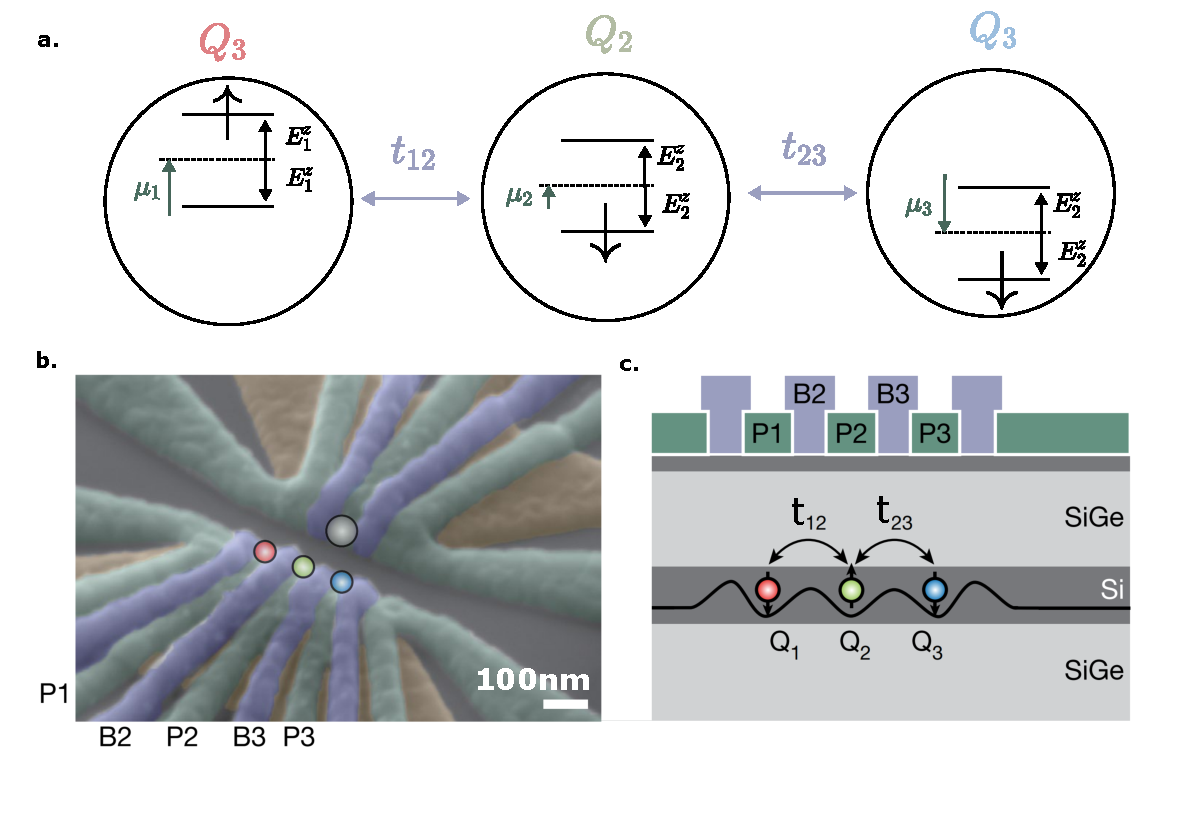
\includegraphics[scale = 0.7]{Figures/3qubithubbard.pdf}
    \caption{\textbf{a.} shows simplified schematic for the important parameters of a Hubbard model: $E_i^z$ the energy splitting due to an applied static field in the $z$ direction; and the inter-dot kinetic coupling $t_{ij}$. The system is shown in the basis state that would be described in second quantisation notation as $c_{1,\uparrow}^\dagger c_{2,\downarrow}^\dagger c_{3,\downarrow}^\dagger\ket{\text{Vac}}$, or more conventionally as $\ket{\uparrow\downarrow\downarrow}$. \textbf{b.} and \textbf{c.} are taken from \cite{Takeda2022}. \textbf{a.} shows a false-colour microgram image of 3 qubit system implemented in a SiGe-Si-SiGe heterostructure. The B lines control the inter-dot couplings whilst the P lines control the chemical potential, and hence occupation, of the dots, as shown in \textbf{c.}.}
    \label{fig:3qubitdiagram}
\end{figure}

Semiconductor quantum dot based processors are a promising platform for building quantum computers. They have several features that make them attractive, of which the most significant are the relatively long decoherence times \cite{Loss2022} and the abundance of manufacturing expertise and infrastructure, which researchers hope will enable rapid scaling of qubit technology once the technology is more advanced. For a review see \cite{Burkard2022}. 

Quantum dot processors are constructed by first growing a semiconductor heterostructure to create a two-dimensional electron gas (2DEG) at the interface between the materials. By applying voltage gates to the surface of the structure the 2DEG can be confined to a sufficiently small region that the electrons behave as if they are in an `artificial atom'; that is, there are a number of well-defined discrete electron energy states on the dot. The number of electrons (up to two per level by the Pauli principle) on the dot can be finely controlled by adjusting those levels relative to the chemical potential of the environment. Such a device with three quantum dots is shown in figure \ref{fig:3qubitdiagram}.

We can control the chemical potentials $\mu_i$ and the inter-dot couplings $t_{ij}$ using the voltage gates on the upper surface of the device. In order to model the device physics, we use the Fermi-Hubbard model \cite{Hubbard1963}, working in the occupation basis. The resulting `Hubbard Hamiltonian' is explained in appendix \ref{appendix:hubbard}.

\section{Quantum error correction}
In classical computers, which are also prone to random errors (a definite $1$ may become a $0$), a variety of error-correction techniques are available \cite{moon_2005}. These are all fundamentally based on the principle of redundancy: that is, if the relevant information is spread over a larger number of bits, than the number of destructive events required to render the state completely unrecoverable is more than one. 

Alas, the no-cloning theorem due to Wootters and Zurek\cite{wootters_1982} proscribes the implementation of straight-forward redundancy-based quantum error correction codes, as the operation
\begin{equation*}
    (\alpha\ket{0_1} + \beta\ket{1_1})\ket{\Psi_2} \rightarrow (\alpha\ket{0_1} + \beta\ket{1_1})(\alpha\ket{0_2} + \beta\ket{1_2})
\end{equation*} is forbidden by quantum mechanics. Additionally, the measurement of a quantum state destroys its superposition. It is therefore difficult to see how a quantum system can be kept in a superposition state through measurements, which inherently act to destroy superpositions.

The solution to this conundrum presents itself in the formalism of stabiliser codes. The key idea to encode our quantum information onto a greater number of qubits than necessary to hold it, and divide the state-space of this new set of qubits into a valid code-space and a larger error-space. The code-space and all error-spaces are each large enough to encode every valid computational state within them, and so that a single error event will push the state out of the code-space and towards the error-space. These are each degenerate subspaces of the measurement outcomes of certain sets of projective measurements called `stabilisers'. Performing these `stabiliser' measurements projects the resulting state precisely into either the code-space - in which case the error is corrected - or the error-space, in which case the error is now precisely known and can be corrected using a known unitary operation. Because the spaces are degenerate, knowledge of which sub-space the state of the system inhabits provides no information as to which valid computational state the system state represents. The original and simplest proposal is the three-bit Shor code, which encodes each qubit in the Hilbert space of three qubits, according to
\begin{equation*}
    \alpha\ket{0} + \beta\ket{1} \rightarrow \alpha\ket{0_10_20_3} + \beta\ket{1_11_21_3}.
\end{equation*} We can then determine if an error has occurred by performing two parity measurements $Z_1Z_2$ and $Z_2Z_3$, and perform an appropriate correction flip. In order to correct a single bit-flip error, that is to defend against the risk of the event
\begin{equation*}
    \alpha\ket{0} + \beta\ket{1} \rightarrow \alpha\ket{1} + \beta\ket{0}
\end{equation*}
we can encode a single computational qubit into a set of three (with the latter two initialised in the state $\ket{0}$) using two \texttt{CNOT} operations:
\begin{equation*}
\begin{aligned}
    & (\alpha\ket{0_1} + \beta\ket{1_1})\ket{0_2}\ket{0_3}\\
      \xrightarrow{\texttt{CNOT(1,2)}} &(\alpha\ket{0_1 0_2} + \beta\ket{1_1 1_2})\ket{0_3} \\
     \xrightarrow{\texttt{CNOT(1,3)}}  &\alpha\ket{0_1 0_2 0_3} + \beta\ket{1_1 1_2 1_3}
\end{aligned}
\end{equation*}
. Here, the code-space is $\spa[\ket{0 0 0}, \ket{1 1 1}]$ (we have dropped the qubit labels). If an error occurs on, say, the second qubit:
\begin{equation}
    \alpha\ket{0 0 0} + \beta\ket{1 1 1} \rightarrow \alpha\ket{0 1 0} + \beta\ket{1 0 1}
\end{equation}
we see that the state of the system has moved into one of three error-spaces: $\spa[\ket{0 1 0}, \ket{1 0 1}]$. We then perform a stabiliser measurement consisting of two projective measurements, \texttt{Z$_1$Z$_2$} and \texttt{Z$_2$Z$_3$}. Our disrupted state is an eigenstate of both of these measurements with eigenvalue $-1$ for both. More generally the error might move the state into a superposition of vectors in more than one of the error-spaces and/or the code-space, in which case these measurements have the virtue of collapsing the state exactly into one or the other subspace. In this case, the only information we gain by the measurement, which consists of the two $-1$ eigenvalues, tells us the system lies in the error-space corresponding to a bit-flip of the second qubit. This is called the \textit{error syndrome}. We can then apply \texttt{X$_2$} to correct the error, all without ever learning the values of $\alpha$ and $\beta$. 
\subsubsection{How the scheme fails}
\begin{figure}[ht]
    \centering
    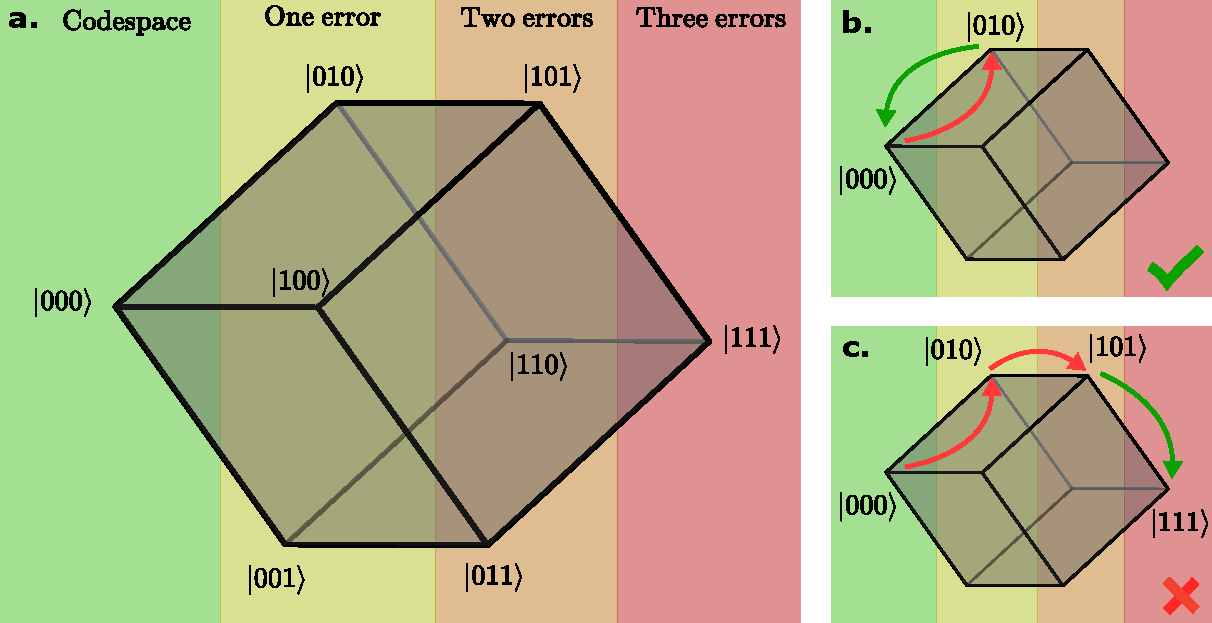
\includegraphics[scale = 0.85]{Figures/cubediagram.pdf}
    \caption{In this figure, the possible states of an error-prone system that starts in the $\ket{000}$ state are represented on the vertices of a cube. Note that the ideal action of the correction flips is to push the system towards either the $\ket{000}$ or $\ket{111}$ states, indicated by the black arrowheads on some edges. \textbf{a.} shows the ideal case of successful error correction. A single error occurs on the second qubit, and a correct pair of parity measurements identifies the error syndrome and applies an $X_2$ correction flip. \textbf{b.} shows how the scheme fails if two errors (or more) occur in the interval between correction iterations: a correctly performed set of parity measurements will result in a correction flip that pushes the qubits further away from the codespace. \textbf{c.} shows how the scheme fails if one error occurs, and the subsequent parity measurements give the wrong result, so an erroneous correction flip (here $X_1$) is applied. On the next round, if no errors occur and the next set of parity measurements is performed correctly, the correction flip will push the state into the $\ket{111}$ error space.}
    \label{fig:cubediagram}
\end{figure}
We can conceptually divide the processes by which the scheme fails into two classes. Firstly there are those that are caused by two or more errors occurring in the time it takes to correct a single error; and those that are caused by an erroneous parity measurement, leading to an applied correction flip. These two processes are illustrated in figure \ref{fig:cubediagram}. This distinction will be referred to again in section \ref{chapter:DQEC}.

\subsubsection{Phase flip errors}

In order to project a general error $\alpha, \beta \rightarrow \alpha', \beta'$ we must also protect against \textit{phase-flips}, that is 
\begin{equation}
    \alpha\ket{0} + \beta\ket{1} \rightarrow \alpha\ket{0} - \beta\ket{1}
\end{equation}
which can be achieved by encoding the triple qubit state here into a trio of qubits in the Hadamard basis $\{\ket{+++},\ket{---}\}$, with $\ket{\pm} = (\ket{0} \pm \ket{1})/\sqrt{2}$ and performing an analogous parity measurement. We can protect against either only bit- or only phase-flips in this way, but protecting against both requires nine qubits in this scheme. It is possible to perform full error correction against both bit and phase flips with just 5 qubits  using a much more complicated encoding scheme\cite{DiVincenzo1996}. The complexity of this 5 qubit scheme means it is unviable using current technology in silicon systems, and we focus on the three-bit bit-flip Shor code for the remainder of the project.


\section{Continuous quantum error correction}\label{sec:CQEC}
One goal of this project is to investigate \textit{continous quantum error correction} (CQEC) schemes, and in particular their application to semiconductor quantum dot qubit devices. 

Continuous quantum error correction refers to a class of error correction schemes that rely on some always-on output signal from the qubit system to gain information about which subspace the qubits inhabit. The original theoretical formulation of these ideas proposed a system of \textit{continuous feedback} to the feedback based on the continuous output signal to reduce drift away from the codespace \cite{Ahn2002}. While there has been some continued development of this theory \cite{Cardona2018}\cite{Cardona2019}, the field has largely moved away from the idea of continuous feedback. Instead, the most promising development has been in an experimental demonstration in superconducting transmon qubits\footnote{These are another promising platform for quantum devices favoured by researchers including groups at Google and IBM. They currently (subject to some controversy) hold the records for the highest qubit counts in quantum devices, and recently claimed to perform a calculation surpassing the capabilities of classical computation `quantum supremacy' \cite{Arute2019}. For a review see \cite{Huang2020}.} of a system which uses a continuous noisy output signal from the qubits to constantly update its `best guess' at the current qubit state, but then applies \textit{discrete} correction flips to move the state back into the codespace when the system is sufficiently confident that an error has ocurred\cite{Dressel2022}. The scheme I propose in section \ref{sec:truly_continuous_theory} also relies on applying discrete correction flips on the basis of a form of continuous measurement. However, the physics of the two devices is very different: in superconducting devices, the two level system that implements a qubit consists of a mode of oscillation of a supercurrent through a Josephson junction, whereas in quantum dot qubits the qubit is implemented as the spin state of an electron. The physical implementation of such a continuous parity measurement is therefore necessarily quite different in the two cases.
\begin{figure}[ht]
    \centering
    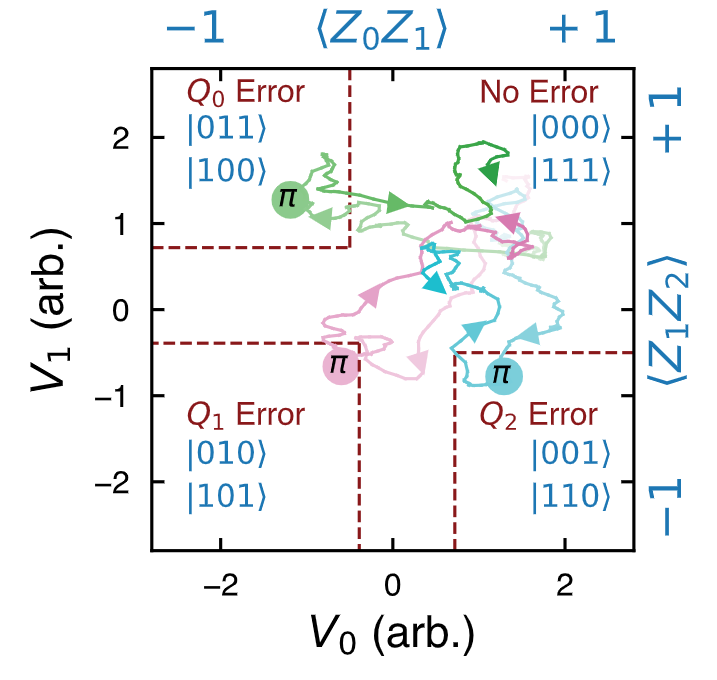
\includegraphics[scale = 0.3]{Figures/dresseldiagram.png}
    \caption{Taken from \cite{Dressel2022}. This diagram shows the principle behind the continuous error correction scheme implemented by Dressel et al., whereby an estimate of the current state of the qubits is continuously updated through two voltage signals that relate noisily to the parity state of the qubits. When threshold is reached (optimised for empirically) where the system decides an error has probably occurred, it performs a correction flip, at which point the signal should drift back into the codespace.}
    \label{fig:dresseldiagram}
\end{figure}


\chapter{Discrete QEC}\label{chapter:DQEC}


\section{Discrete error correction schemes using repeated parity measurements} \label{sec:repeat_analysis}
This section develops a framework for analysing error correction schemes based on discrete, but rapidly repeated, parity measurements and correction flips. This analysis is motivated by experimental demonstrations of repeated non-demolition measurements\footnote{`Non-demolition' means that the collapsed state that results from measurment remains available to the experimenter.} in silicon systems \cite{Xue2020} and \cite{Nakajima2019}. The former make use of Elzerman readout\cite{Elzerman2004} while the latter applies the emerging technology of singlet-triplet readout using radio frequency reflectometry \cite{Oakes2022}. The analysis will then be used to conclude that bit-flip error-correction schemes implemented using current techniques are limited in their performance only by the fidelity of the readout, and not by the readout speed or the rate of occurrence of errors. This is not true for phase-flip correction. 

\section{Markovian analysis of discrete error correction}
The analysis presented here allows for the efficient and exact calculation of the expected fidelity of such a scheme given certain characteristic parameters: the rate of errors, the frequency of error correction cycles, and the fidelity of the error syndrome measurements.
More details regarding the theoretical treatment of decoherence processes are given in appendix \ref{appendix:decoherence}. Appendix \ref{appendix:decoherence} also derives the result that is crucial to the analysis: that all standard decoherence processes have the property that, when they are applied to a diagonal density matrix representing our knowledge of the system state, the result is another diagonal density matrix. This means that by choosing a basis where the initial (codespace) state of the system is one of the basis vectors, we can analyse the system density matrix as a vector, and apply Markovian evolution by calculating the relevant transition matrix. 

Here I model the effects of a process of repeated error-correction scheme for mitigating bit-flip errors, but the process is very similar for correcting phase-flip errors. The system is initially prepared in the state $\ket{\psi} = \alpha \ket{0} + \beta \ket{1}$, whose fidelity we want to maintain for as long as possible. We can apply CNOT operations between this and two further code qubits to obtain $\alpha \ket{000} + \beta \ket{111}$. Using a change of basis technique with some subtleties that are detailed in appendix \ref{appendix:changeofbasis}, we can write any such state to be protected in the `analytical basis' as $\ket{000}$.

\section{Correction scheme}
\begin{figure}[ht]
    \centering
    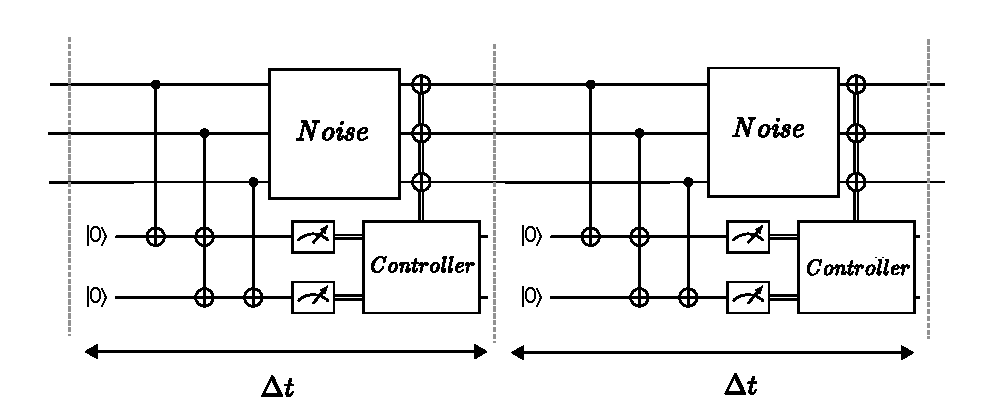
\includegraphics[scale = 0.9]{Figures/Circuit/diagram.pdf}
    \caption{Circuit diagram of the repeated noise and error-correction model examined in this section. The majority of time is spent in the measurement phase, with the operations on either side being much faster. The controller takes in the results of the two parity measurements and determines the best correction flip to apply to the code qubits.}
    \label{fig:circuitdiagram}
\end{figure}
    
The correction scheme modelled here is the standard three-bit parity code. We assume errors accumulate for time $\Delta t$. At the end of this period, a combination of H and CNOT gates is applied to encode the parity state of the three qubits onto two ancilla qubits. These qubits are read out for time $\Delta t$, during which more errors accumulate. At the end of this period, two operations are performed in quick succession: first any correction flips that are required to undo errors detected in the previous cycle are performed, and secondly the ancillas are rotated back to $\ket{0}$ and encoded with the new parity state of the qubits. Since X gates all commute with each other, it does not matter if previous errors are corrected after new errors have occurred, so long as they are corrected before the new set of errors is loaded onto the ancillas for readout. This scheme is shown in figure \ref{fig:circuitdiagram}.

In appendix \ref{appendix:markovanalysis}, it is derived that the evolution of this state over one cycle can be written as 
\begin{equation*}
    \mathbf{P}(t + \Delta t) = CE\mathbf{P}(t),
\end{equation*} where $\mathbf{P}$ is a vector describing the on-diagonal terms of the state density matrix, and C and E are matrices:
\begin{align*}
    E &=     
    \begin{bmatrix}
        q^3& q^2p& q^2p& qp^2& qp^2& p^3 \\
        2 q^2p& qp^2 + q^3& 2 qp^2& 2 q^2p& p^3 + q^2p& 2 qp^2\\
        q^2p& qp^2& q^3& p^3& q^2p& qp^2\\
        qp^2& q^2p& p^3& q^3& qp^2& q^2p\\
        2 qp^2& p^3 + q^2p& 2 q^2p& 2 qp^2& q^3 + qp^2& 2 q^2p\\
        p^3& qp^2& qp^2& q^2p& q^2p& q^3\\
    \end{bmatrix}\\
    C &= 
    \begin{bmatrix}
        F_0^2 & F_0 F_1 & F_1^2 & 0 & 0 & 0 \\
        2F_0'F_0 & F_0 F_1' & 0 & 2F_1 F_1' & F_0' F_1 & 0\\
        F_0'^2 & 0 & F_1'^2 & 0 & F_0' F_1' & 0 \\
        0 & F_0' F_1' & 0 & F_1'^2 & 0 &F_0'^2 \\
        0 &F_0' F_1 & 2F_1' F_1&0&F_0F_1'&2F_0'F_0 \\
        0&0&0& F_1^2 &F_0 F_1 & F_0^2
    \end{bmatrix}.
\end{align*} Here $p = 1-q = \frac{1}{2}(1-e^{-\Delta t /T_{\text{err}}})$ (see appendix \ref{appendix:decoherence}), and $F_1 = F_1(\Delta t)$ and $F_0 = F_0(\Delta t)$ are the probabilities of correctly measuring an even or odd parity state respectively, which will typically depend exponentially on the readout time. It is clear from the symmetry of the matrix that the system will eventually equilibrate into a steady state where each state has equal occupation to its all-bits-flipped counterpart.

\section{Using flow analysis to investigate error regimes}
Intuitively, there are two ways in which the error correction scheme can fail. Firstly, error flips could occur on two or more of the qubits, for example $\ket{000} \longrightarrow \ket{110}$. Then a successful set of parity measurements will push the state into the error space, in our example $\ket{110} \longrightarrow \ket{111}$. The whole mechanism takes only one cycle of errors and corrections, and I call this a \textit{direct} error process. One supposes there may well be a parameter space in which this is the dominant mechanism for loss of qubit fidelity; this I call the \textit{error-limited} regime.

Secondly, a single qubit flip could occur, for example $\ket{000} \longrightarrow \ket{001}$. If the subsequent fidelity measurements give the wrong outcome (e.g. odd-even), the correction step may push the state over into the error space, $\ket{001} \longrightarrow \ket{101}$. The most likely outcome of the next round of errors and correction is then $\ket{101} \longrightarrow \ket{111}$. Similarly, there could be no error flips but two erroneous parity measurements in a row. These are both two-step, or \textit{indirect} error mechanisms. A regime in which this is the dominant source of errors I call the \textit{readout limited} regime.

In figure \ref{fig:cubediagram}, the process indicated by \textbf{b.} would belong in the first category, and the process in \textbf{c.} in the second.

In theory there is a third two-step process that starts with a single error flip, which is not corrected by the correction step, and is followed by a further flip on the next round of errors. This turns out to never dominate the loss of qubit fidelity, and nor does any more complicated process.

We can explore these different regimes by examining the rate of flow of probability through the system throughout the lifetime of a qubit - that is, over the time the system takes to equilibrate between the codespace $\ket{000}$ and the `anti codespace' $\ket{111}$. The net probability flux through the system from state $j$ to state $i$ during step $n$, at which point the probabilities are given by the vector $\mathbf{P^n}$, is given by
\begin{equation*}
    J_{ij} = M_{ij}P^n_j - M_{ji} P^n_i
\end{equation*}
or in matrix notation
\begin{equation*}
    J = M\mathbf{P^n} - (M \mathbf{P^n})^\mathrm{T}
\end{equation*}.

Then we define \textit{direct flow} as $J_D = J_{5,0}$, that is, the rate at which states jump in one step from $\ket{000}$ to $\ket{111}$. This corresponds with the error-limited case above. \textit{Indirect flow} is given by $J_I = J_{5,3} + J_{5,4}$, and is the rate at which states arrive at $\ket{111}$ via $\ket{110}$, $\ket{101}$ and $\ket{011}$. Then we have other flow $J_O = J_{5,1} + J_{5,2}$. Note that we have $\dot{P_5} = J_D + J_I + J_O = J_\mathrm{total}$, as required by conservation of probability.

We can fix the parity readout fidelities $F0 = F1 = F$ (= 0.99), and vary the error probability $p$. For each $p$, we start the system in $P^0_i = \delta_{i,0}$, and apply $M$ until the fidelity falls below some threshold (here 0.51). At each time step we calculate $J_D$, $J_I$ and $J_O$. Then we can plot the ratios $\int J_D/J_\mathrm{total}dt $, etc. We can repeat the experiment holding $p$ fixed and varying $F$. The results are shown in figures \ref{fig:flowprop1} and \ref{fig:flowprop2}. We find that using different fixed values of $F$ and $p$ produces a very similar plot. In each case, we see a clear point of crossover between the error- and readout-limited regimes around the point $p = 1-F$, that is, the point at which the probability of an error flip is comparable to the probability of an incorrect parity readout. Where $p \gg 1-F$, the system is firmly in the error-limited regime, whereas for $1-F \gg p$, it is in the readout-limited regime. Around the middle point probability appears to flow without preference through all of the routes available.
\begin{figure}[ht]
    \centering
        \centering
        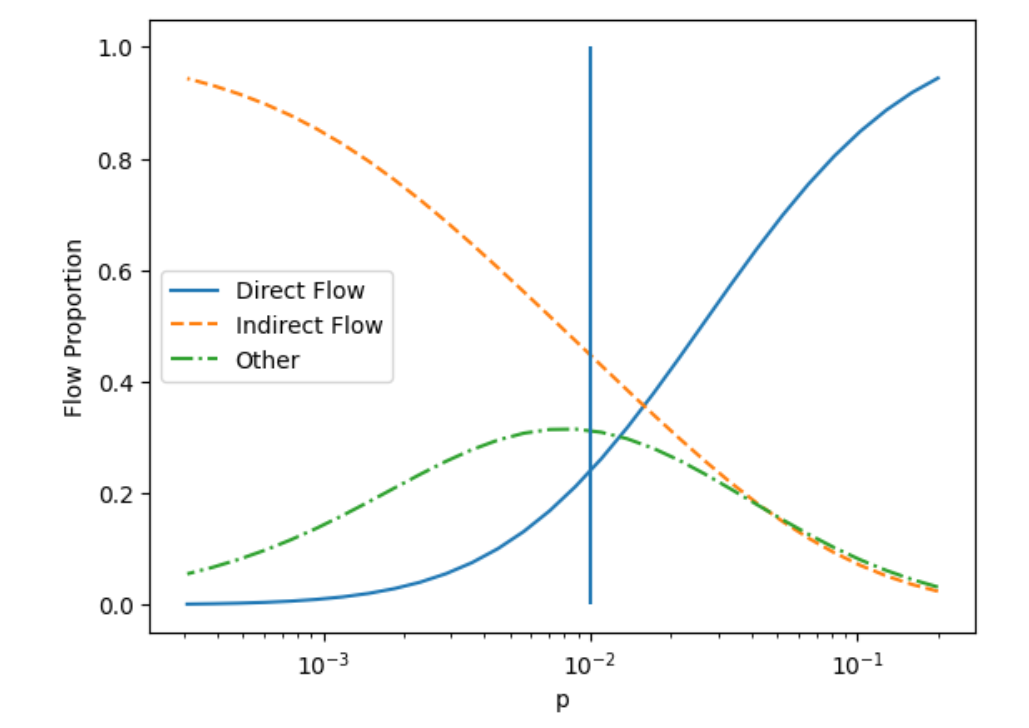
\includegraphics[width=0.6\textwidth]{Figures/flow/f_fixed.png} % first figure itself
        \caption{Proportion of direct, indirect and other flows (as defined in the text) as a function of $p$ with $F = 0.99$. Note the logarithmic scale. The vertical line indicates $p = 1-F$.}
        \label{fig:flowprop1}
\end{figure}
    
\begin{figure}[ht]
        \centering
        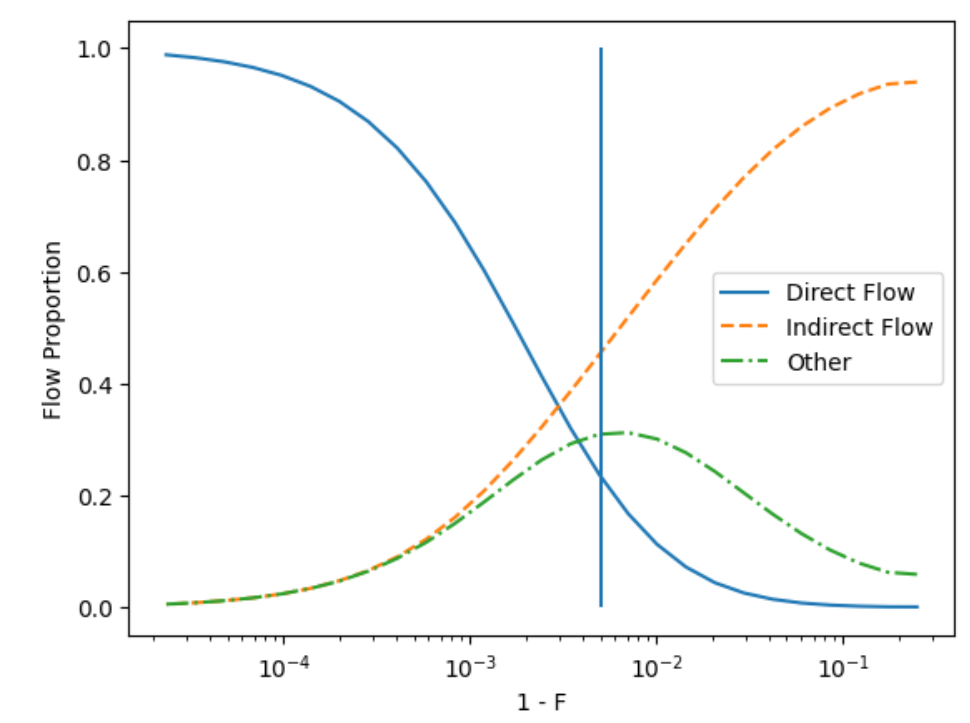
\includegraphics[width=0.6\textwidth]{Figures/flow/p_fixed.png} % second figure itself
        \caption{Proportion of direct, indirect and other flows (as defined in the text) as a function of $1-F$ with $p = 0.01$ fixed. Note the logarithmic scale in $1-F$. The vertical line indicates $p = 1-F$.}
        \label{fig:flowprop2}
\end{figure}

\section{Understanding the state of error correction in silicon using the analysis}
The transition matrix allows us to gain some insight into different error regimes: one where the rate of equilibration out of the codespace is dominated by the process of two errors occurring in one timestep - the \textit{error-limited regime}, and another where it is dominated by erroneous correction flips caused by incorrect parity measurements - the \textit{readout limited} regime.  These results allow for a simple understanding of certain experiments. For example, in \cite{Cramer2016}, not silicon quantum dot qubit but rather a nuclear spin qubit experiment, the fidelities are given as $F1\approx0.999$, $F0\approx0.9$, with a quoted $T_2^*$ time of around $12\unit{\milli\second}$ (all three quantities in fact vary from qubit to qubit). Given these parameters, the model gives a reasonable estimate of the fidelity of the error-corrected qubit, remaining within 10\% of the measured fidelity for the duration of the experiment. These parameters are such that the experiment is occurs in the `intermediate regime' $p_{\text{err}}\sim 1-F$(see appendix \ref{appendix:flowanalysis}), which means that both reducing the error rate per step and increasing the readout fidelity would have an appreciable impact on the long-term fidelity of the qubit. 

In silicon, however, the rate of bit flip errors and the repetition cycle time of error correction means that $p \ll 1-F$. As an example of Elzerman readout, in \cite{Xue2020} a bit-flip $T_1$ time of 50\unit{\milli \second} is reported, with a readout cycle time of 475 \unit{\micro\second}, so that $p \approx 0.005$, whereas they report a single-shot measurement fidelity of 75\%. For bit-flip errors, they are firmly in the readout-limited regime. However, dephasing times in these systems can be up to hundreds of \unit{\micro\second}, so if this kind of measurement were applied to error correction the resulting error-correction be in the intermediate regime.

RF reflectometry techniques allow much faster readout with potentially higher fidelity. The repeated spin-basis measurements in \cite{Nakajima2019} on a quantum dot system are performed at a repetition rate of around $7\unit{\micro\second}$, whereas the relaxation time is measured on the order of $1-3\unit{\milli\second}$, and the reported measurement fidelity is on the order of around $0.6$.  Despite the increase in fidelity, the speedup in measurement times means that for bit-flip errors the use of such technology would still be readout-limited. The difference with RF reflectometry techniques is that with faster readout, even phase-flip protection will likely be readout-limited. 

This analysis leads us to the conclusion that the field should focus as a matter of priority on improving the fidelity of non-demolition measurements in order to improve qubit coherence times through error correction. This will have more of an impact than improving readout time or improving the natural coherence times $T_1$ and $T_2^*$. Only if measurement fidelities reach $\sim 99\%$ for phase-flip errors, and at least $\sim99.9\%$ (probably higher) for bit-flip errors, will the performance of QEC be limited by the rate of naturally occurring errors.

\chapter{Continuous QEC using RF reflectometry techniques} \label{chapter:CQEC}
\begin{figure}[ht]
    \centering
    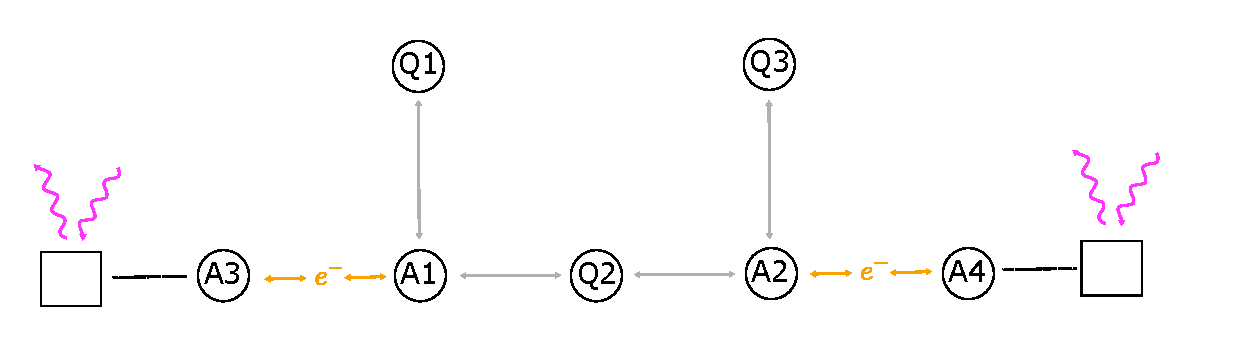
\includegraphics[scale = 0.9]{Figures/7q.pdf}
    \caption{Schematic of the layout of qubits for the continuous error correction scheme. Q1, Q2 and Q3 comprise a single logical qubit. A1 to A4 are ancilla qubits used to detect bit flip errors in the logical qubits. Q1 and Q2 are continuously weakly coupled to A1 through a tunnel barrier, and likewise Q2 and Q3 to A2. R1 and R2 are resonators, which are additional quantum dots held at a higher electron occupancy than the qubits. These are probed using RF signals, and their coupling to the charge on the ancillas then allows the singlet/triplet state of the ancillas, as in \cite{Oakes2022}.}
    \label{fig:7qubitlayout}
\end{figure}
\section{Scheme summary}

In this section a proposal for continuous error correction is developed\footnote{I thank Chris Long, Dr Mertig, Giovanni Oakes and my supervisor Dr Arvidsson-Shukur for contributing variously to the development of the ideas presented here.}. Recent developments in the field of RF reflectometry measurements enable the measurement of the singlet/triplet state of two adjacent qubits coupled via a tunnel barrier, by monitoring the RF reflection characteristics of a neighbouring electron reservior \cite{Oakes2022}. The codespace qubits are to be coupled pairwise to two ancilliary qubits whose function is to perform parity measurements, in such a way that any deviation from the codespace will result in a change of state of one or both of the ancilla qubits, depending on the error syndrome. The rate at which the error propagates to the ancilla qubit(s) is in the tens of nanoseconds, a faster timescale than either gate times (hundreds of nanoseconds) or readout (the state of the art \cite{Oakes2022} achieves 6\unit{\micro\second}).

This scheme is potentially more efficient than a repeated error correction scheme like those analysed in section \ref{sec:repeat_analysis}. One reason for this is that the `dead time' after an error has occurred during which the system is vulnerable to a second error is limited by the time for the ancilla to be reset, which is also on the order of microseconds (e.g. see \cite{Nakajima2019}). A second, more significant advantage is that the scheme does not require any quantum gates to be performed for the purposes of error syndrome detection, as such detection happens continuously and simultaneously with circuit gates. This reduces circuit complexity, and avoids the error accumulation associated with performing the syndrome measurements. However, I conclude that, at least with present technology, it is unlikely to provide a practical means of improving qubit fidelity (see section \ref{sec:feasibility}).


The proposed qubit layout is given in figure \ref{fig:7qubitlayout}. The nature of the circuit requires a 2D array of quantum dot structures, of which there is not yet any published experimental demonstration, but a proposed architecture was proposed in \cite{Tadokoro2021}. In the scheme as analysed here, the logical qubit is encoded in the \textit{odd-odd parity subspace} of three qubits Q1, Q2, and Q3. Any of the four subspaces (even-even, even-odd, odd-even, odd-odd) may be used as codespaces with a modified scheme, as explained in appendix \ref{appendix:evenparitycodespace}. There are two pairs of ancilla qubits: A1, A3, and A2, A4. Each of these is initially prepared in the $T_0$ triplet state. As shown in the figure, each pair of qubits Q1 and Q2, Q2 and Q3, is weakly coupled to one ancilla qubit through a voltage-controlled tunnel barrier. If the couplings are sufficiently well-tuned, the ancilla qubits will remain as triplets and no tunneling will occur. When a bit-flip error occurs on one of Q1, Q2 or Q3, this will cause one or both (depending on the error syndrome) of the ancilla pairs to rotate into a singlet state. This allows (subject to complexities discussed in section \ref{sec:tunneling_question}) tunneling between the electrons in the affected pair, which is registered as a change in dispersive response of the nearby resonator. Thus the error syndrome is immediately detected as a signal in the continuously monitored reflectometry circuit.

\section{Theoretical treatment of scheme with second order perturbation theory}
 In appendix \ref{appendex:perturbationtheory} the behaviour of this system is predicted using second order perturbation theory. The results are:
 \begin{itemize}
    \item as long as the system remains in the codespace, both pairs of ancilla qubits will rotate into singlets at frequency $\delta$ set by the inhomogeneities in the qubits potentials and Zeeman splittings. This frequency must be lower than the rate of errors for the scheme to have a positive impact on the lifetime of qubits.
    \item  When a bit-flip error ocurrs on one of the code qubits, one or both of the ancilla pairs will rotate into singlets at a frequency $2\Lambda_t = 4t^2/U$, where $t$ is the coupling strength between the qubits and $U$ is the on-site coulomb repulsion. The analysis treats the variation in these quantities from site to site as small.
 \end{itemize}

 \section{Numerical simulation of the scheme}
 In order to validate the predictions of the theoretical analysis above, and as the basis for a more advanced simulation that will predict its fidelity and behaviour under a continuous noise model, I wrote a software package that could simulate such quantum dot systems. There were multiple challenges related to the technical complexity and performance requirements of the code, and its development is detailed in appendix \ref{appendix:software}. To demonstrate the capabilities of the simulator, some simple circuits and the results of a benchmarking exercise are shown in figure \ref{fig:benchmark}.
\begin{figure}[ht]
    \centering
    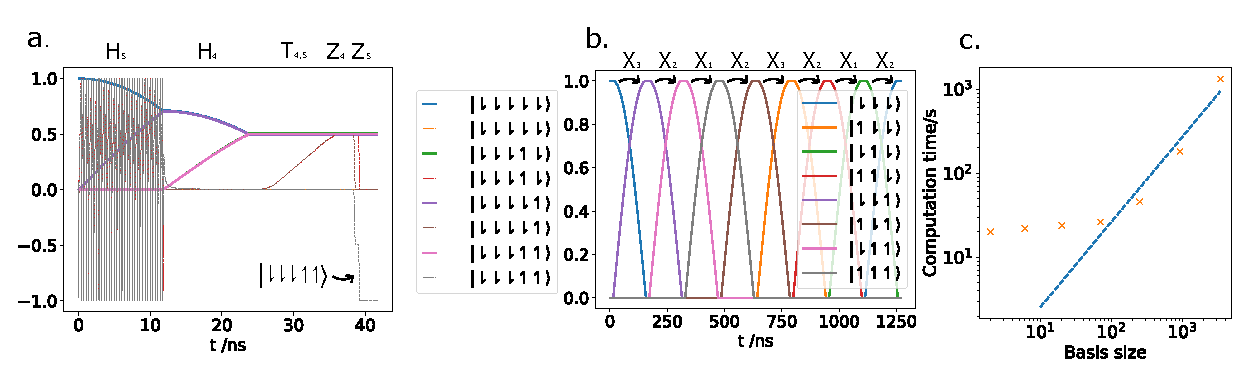
\includegraphics[scale = 0.85]{Figures/benchmark/benchmarks.pdf}
    \caption{Testing the capabilities of the simulation software. \textbf{a.} A plot of 5-qubit system showing the amplitudes (solid lines) and phases (dashed lines) of significant basis states. The plot demonstrates of a CPHASE gate acting on the last two qubits, so that the $\ket{\downarrow\downarrow\downarrow\uparrow\uparrow}$ state acquires a phase shift of $\pi$. First an X gate is applied to each of the two qubits, then a coupling between them is applied, and finally a z-rotation is applied by increasing the static field\protect\footnotemark. \textbf{b.} A sequence of X flips on a 3-qubit system. This circuit is generalised to N qubits to benchmark the simulator, with results given in \textbf{c.}. The results indicate a consistent speed of around 7.5 million statevector derivative elements calculated per second.}
    \label{fig:benchmark}
\end{figure}
\footnotetext{Applying a Z unitary rotation is not a capability typically built into such processors as it is unnecessary due to a technique called $Rz$ delaying (see, e.g. \cite{Nielsen2010} chapter 4.), but I implement it here to make the operation of the CPHASE clearer.}

\section{Energy shifts due to hopping coupling}

\begin{figure}[ht]
    \centering
    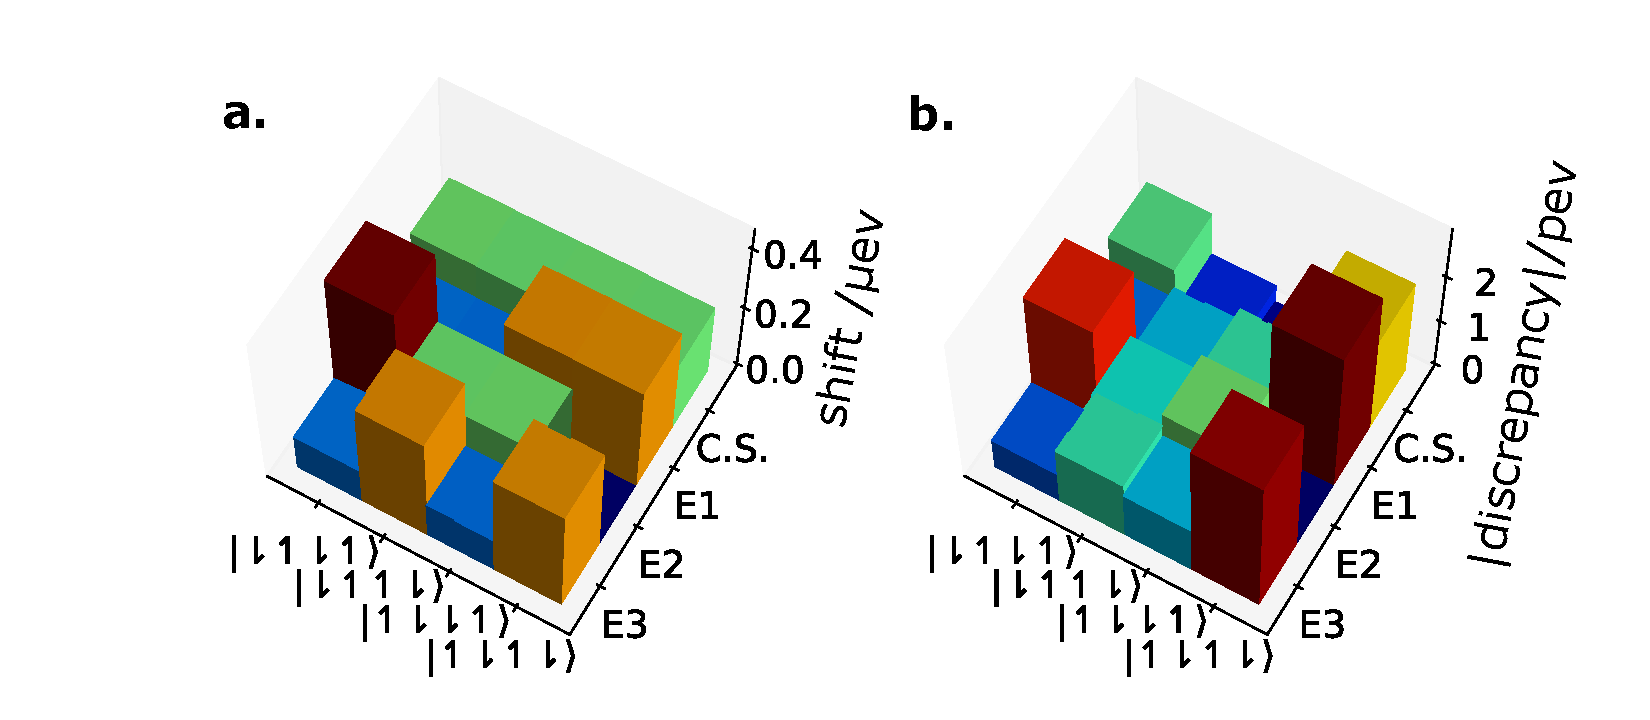
\includegraphics[scale = 0.4]{Figures/shifts.pdf}
    \caption{\textbf{a.} shows the calculation of energy shifts of the various relevant computational basis states calculated with a coupling of $0.015\unit{\milli\electronvolt}$ applied. Only one branch $\ket{\uparrow\downarrow\uparrow}$ of the computational state in each subspace is shown. This can be compared with the second order perturbation theory result calculated in table \ref{table:shifts}. The (absolute value of) the discrepancy between the simulation and the perturbation theory result is given in \textbf{b.}. Note the scale in the second plot.
    \label{fig:shifts}}
\end{figure}
It is important to know the energies of the perturbed computational states for two reasons: firstly, in order to validate the second-order perturbation theory results in appendix \ref{appendix:perturbationtheory}; and secondly knowing the exact energies of these states is important if one is to use oscillating microwave signals to drive transitions between the states, to implement unitary rotations on the qubits while the coupling is active.

I find these by the following procedure: we initialise the system in the computational basis state of interest, and the Hamiltonian with all couplings zero. Then I perform an interaction picture simulation where the couplings are ramped up to the steady state value over a time period that is sufficiently long to ensure adiabatic evolution of the state ($100\times\braket{U_i}^{-1}$ as this is the shortest timescale in the system). I compare this state to a list of the eigenvectors of the matrix generated by the Hamiltonian with the coupling at full strength. The eigenvector which has the maximal inner product with this state (the inner product is close to unity for the correct state, and close to zero otherwise) is the perturbed eigenvector associated with the original state in the computational basis state, and we take the associated eigenvalue as the perturbed energy.

The results for a coupling of 0.015\unit{\milli\electronvolt}, which is slightly higher than a typical coupling, and other typical experimental parameters, are given in figure \ref{fig:shifts}. The simulation agrees with the perturbation theory calculation within 1\%. The agreement is closer for smaller coupling values.

\section{Demonstrating the error propagation from code qubits to ancilla qubits}
We now want to demonstrate the process of propagation by which bit-flip errors in the code qubits Q1, Q2, Q3 result in the relevant ancilla pairs rotating into singlets, or in the reduced basis approximation described in \ref{sec:reduced_basis_approx}, the qubits A1 and A2 rotating from $(\ket{\uparrow} + \ket{\downarrow})/\sqrt{2}$ to $(\ket{\uparrow} - \ket{\downarrow})/\sqrt{2}$, which is approximately equivalent.

We can achieve this by initialising the code qubits in the codespace, and then adiabatically turning on the coupling. We let this system run in steady state for enough time to establish the rate at which the singlets are introduced in the codespace. We then instantaneously apply an X unitary on one of the qubits by, and continue to let the simulation run. Afterwards, we can project the resulting time-evolved statevector data into the singlet and triplet spaces. The system prior to the bit flip is shown in figure \ref{fig:beforeflip}, and the behaviour when a bit-flip is introduced mid-way through the simulation is shown in figure \ref{fig:afterflip}.
\begin{figure}[ht]
    \centering
    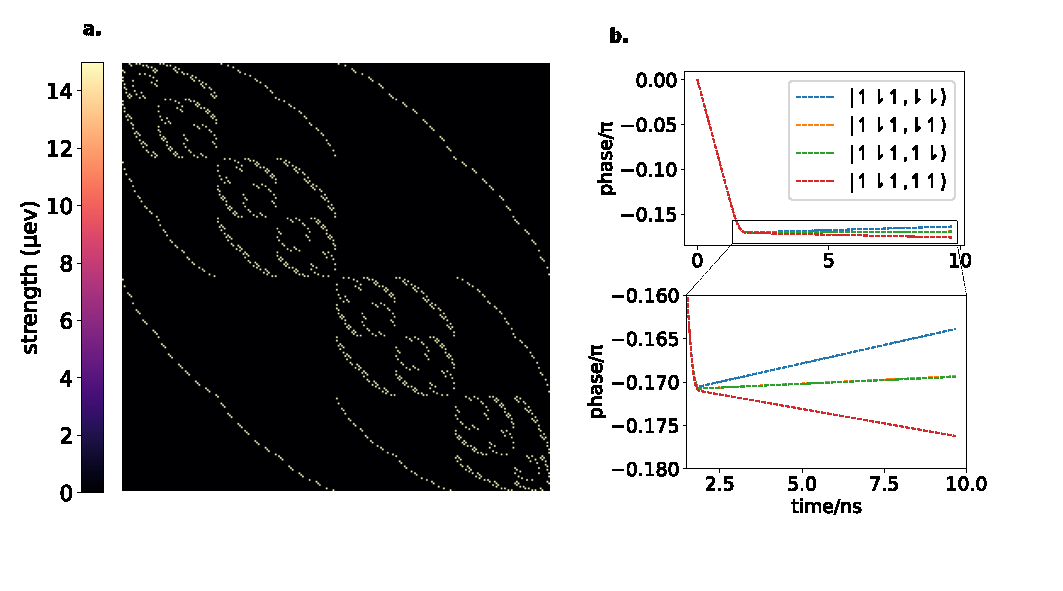
\includegraphics[scale = 1]{Figures/singlettriplet.pdf}
    \caption{The effect of applying the hopping coupling to the system whilst still in the codespace. \textbf{a.} shows the (elementwise absolute value of the) hamiltonian matrix in the interaction picture at full strength. \textbf{b.} shows the rate of aquisition of phase of the relevant basis states. The phase initially drops when the coupling is applied, and then the states slowly drift apart from one another in phase due to the difference in electron g-factor of around 30 \unit{\mega\hertz}. At this rate, the triplet will `flip' into a singlet after around 200 \unit{\nano \second}, so this combination of parameters (coupling strength = 0.015 \unit{\milli\electronvolt}) is not be suitable for error correction. The inhomeneity between the sites needs to be reduced.
    }\label{fig:beforeflip}
\end{figure}

\begin{figure}[ht]
    \centering
    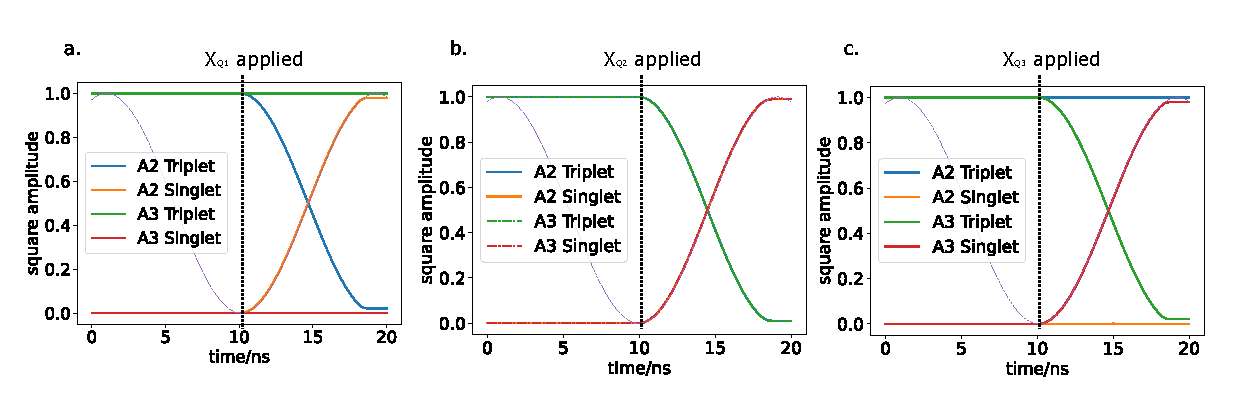
\includegraphics[scale = 0.87]{Figures/flips.pdf}
    \caption{Demonstrating the expected behaviour of the ancillas when a bit flip error is artificially introduced on one of the code qubits: Q1 is flipped in \textbf{a.}, resulting in a rotation of the A2 ancilla; Q2 is flipped in \textbf{b.}, resulting in \textit{both} A2 and A3 rotating, and Q3 is flipped in \textbf{c.}, so that A3 rotates only. In each case, the purple dashed line shows the expected frequency of rotation derived in section \ref{sec:truly_continuous_theory}, $\Lambda_t$. The dotted purple line shows the arbitrarily set threshold for detection. Note that the period of rotation is much faster than the other typical timescales of quantum dot qubit systems.
    }\label{fig:afterflip}
\end{figure}

\section{Future work required}
It is unfortunate that I developed the idea for how to implement CQEC in semiconductor quantum dot devices quite late into the course of my investigation, which left time only for limited analysis and simulation of the scheme. At the time of writeup, I am in the process of extending my simulation software to include the capability to condition the applied gates on the results of mid-circuit measurement; to perform the state collapse associated with such measurements; and to include a noise model. This means the behaviour of the full scheme with dynamically applied correction flips can be simulated under the constant application of noise. I hope that upon completion, this software will allow me to more fully understand the behaviour of the scheme in noisy conditions and provide better bounds on the required physical parameters. The physics of singlet/triplet tunneling under continuous conditions and in a superposition with a small singlet component also need to be better understood to properly analyse the scheme.


\section{Feasibility of the scheme}\label{sec:feasibility}
Despite these limitations of the numerical analysis up to this point, we can draw some tentative conclusions about the likely feasibility of the scheme as it is presented here. There are features of this scheme which are potentially attractive, such as the fact that it does not require error correction steps to be programmed into a circuit, and the essentially instantaneous error detection that should lead to reduced `dead time'. However, the above proposal is unlikely to be practical as a means of increasing electron fidelity with current experimental parameters. 

The main problem with this scheme is that it only provides a way to protect against bit flip errors. The typical coherence time for such `relaxation' processes, $T_1$ in silicon systems is typically in the hundreds of microseconds or a few milliseconds \cite{Loss2022}\cite{Zwerver2022}; the best performance in this respect is isotopically purified $^{28}$Si, in which all atomic nuclei have zero spin. The more pressing limitation for such systems are phase-flip errors, whose coherence times $T_2^*$\footnote{$T_2^*$ is the `effective' decoherence time taking into account unknown but constant inhomogeneities in the system and applied field, whereas $T_2 > T_2^*$ is for decoherence cause by purely random environmental noise. $T_2^*$ is normally the more relevant quantity.} are typically 1-3 orders of magnitude shorter \cite{Loss2022}. I can see no obvious way to extend the scheme as described here to phase-flip errors. The issue is that most discrete error corrections can make use of the fact that phase- and bit- flip errors are equivalent up to a change of basis $\ket{0} \leftrightarrow \ket{+}$, $\ket{1}\leftrightarrow\ket{-}$, and just transform into the appropriate basis before the error correcting step using Hadamard gates. This is not possible in a continuous scheme like the one described here.

Even if we restrict ourselves to trying to reduce errors due to relaxation and leave phase-flip correction to other techniques, there are still limitations due to the inhomogeneities of silicon systems. In order for the correction to provide an improvement to the current $T_1$ times of order milliseconds, the time it takes the ancillas rotate into singlets whilst the system is in the codespace longer than this. This requires the overall spin difference $\delta_{A1, A3} = E_{A1}^z - E_{A3}^z$ and $\delta_{A2, A4}$ to be significantly less than $1/T_1 \approx 1\unit{\kilo\hertz}$, which is smaller than the expected range \cite{Hwang2017}.

During the course of the project I also developed a highly theoretical error-correction scheme that in principle could correct against both phase flip and bit-flip errors. This I describe in appendix \ref{appendix:lockedstates}.

\chapter{Conclusions}
I have presented an overview of the current state of discrete QEC, and applied a Markovian analysis to demonstrate the existence of two regimes in which the error is limited by readout fidelity or by the rate at which errors naturally occur. Consulting current experimental work allows me to draw the following conclusion: in order to improve the ability of such schemes to maintain qubit fidelity for as long as possible, both with standard Elzerman readout and with more recent EF reflectometry techniques, the fidelity of non-demolition measurements must be improved. This will impact the maintenance of qubit fidelity more than the improvement of measurement speed or the inherent qubit coherence times.

Secondly, I have proposed a continuous error correction scheme in a semiconductor system using RF reflectometry to detect errors immediately after they occur. I have applied a perturbation theory analysis to show how the system would work in the ideal case, and developed a simulation code to verify these predictions, but still in somewhat idealised conditions. It appears that current semiconductor qubit devices have too high an imhomogeneity between qubits to support the idea. Further work on the simulator will allow me to simulate the scheme in more realistic conditions to more fully evaluate its ability to keep qubits in the desired codespace.

\begin{appendices}\label{appendix:parameters}
\chapter{Table of orders of magnitude of physical parameters}
\begin{table}[ht]
    \centering
\begin{tabular}{|c|c|c|c|}
    \hline
    Parameter & Symbol & Range & Example Reference\\
    \hline
    On-site coulomb repulsion & $U_i$ & $\sim 1\mathrm{Ry} \sim$ 1-10 \unit{\milli\electronvolt} & \cite{Shim2022}\\
    \hline 
    Static magnetic ($z$) field & $B_i^z$ & 1 - 10 \unit{\tesla} & \cite{Jock2018} \\
    \hline
    Variation in electron g factor & $\delta B_i^z$ &0.01 - 0.1 \unit{\mega\hertz} &\cite{Hwang2017} \\
    \hline
    Hopping coupling strength & $t_{ij}$ &$0.001 - 0.01$ \unit{\milli\electronvolt} & \cite{Veldhorst2015} \\
    \hline
    Phase flip coherence time &$ T_2^*$ &$1$\unit{\micro\second} - $500$\unit{\micro\second}& \cite{Loss2022}\\
    \hline
    Bit flip coherence/relaxation time &$T_1$&$1\unit{\milli\second}$ - $1\unit{\second}$& \cite{Xue2020}\\
    \hline

\end{tabular}
\caption{Table of the orders of magnitude of the key physical parameters of current silicon qubit technology, along with example references.}\label{table:parameters}
\end{table}
\chapter{The Fermi-Hubbard model of interacting quantum dots}\label{appendix:hubbard}

We model the multiple quantum dot system in the second-quantised `Fock' or `occupation' basis using the Hubbard model\cite{Hubbard1963}. 
We parameterise the model with several key parameters. $\mu_i$ are the chemical potentials at each site, which are set primarily by the voltages applied directly to the dots, for example using the $Pi$ lines in figure \ref{fig:3qubitdiagram}. $E^z_i$ are the Zeeman energy splittings associated with the $z$ component of an applied static magnetic field and the $U_i$ are terms representing same-site coulomb repulsion. For example, the state $\ket{\uparrow\downarrow\downarrow}$ is $2E_1^z$ higher in energy than the state $\ket{\downarrow\downarrow\downarrow}$. The state $\ket{\updownarrow\varnothing\downarrow}$, with two electrons on the first site and none on the second is around $U_1$ higher in energy than either, with $U_i \gg E_i^z$. In second quantisation we write the uncoupled part of the Hamiltonian as
\begin{equation*}
    \hat{H_0} = -\sum_{i = 1}^{N}{\sum_{\sigma \in \{\uparrow, \downarrow\}}{\mu_i\hat{n}_{i\sigma}}}
\end{equation*}
\begin{equation*}
    +\sum_{i = 1}^{N}{(\frac{E_i^z}{2} (\hat{n}_{i\uparrow} - \hat{n}_{i\downarrow}) 
    + U_i \hat{n}_{i\uparrow} \hat{n}_{i\downarrow}) }.
\end{equation*}

The addition of kinetic coupling terms, which are controlled by the inter-dot gates (e.g. the $Bi$ lines in figure \ref{fig:3qubitdiagram}) results in a further set of terms
\begin{equation*}
    \hat{H_J} = -\sum_{i < j}t_{ij}{\sum_{\sigma \in \{\uparrow, \downarrow\}}
    (\hat{c}_{i,\sigma}^\dag \hat{c}_{j\sigma} + \hat{c}_{j,\sigma}^\dag \hat{c}_{i\sigma})}
\end{equation*} with $t_{ij}$ the coupling between the $i$th and $j$th site, given by\begin{equation*}
    t_{ij} = \bra{\phi_i}\frac{\hat{p}^2}{2m^*}\ket{\phi_j}.
\end{equation*} A change to these parameters is called a `pulse'. The other means of control we have over the system is to apply microwave radiation of given amplitude $\Omega$ and phase $\gamma$. This results in a last Hamiltonian component for what we call a `drive':
\begin{equation*}
    \hat{H}_\omega = -\Omega(t)\cos(\omega t + \gamma) \sum_{i = 1}^{N}\sum_{\sigma,\xi \in \{\uparrow, \downarrow\}}
    \frac{\mu_b g_j}{2}\mathbf{B}\cdot\mathbf{P_{\sigma\xi}}\hat{c}^\dag_{i\sigma}\hat{c}_{i\xi}
\end{equation*}.
These microwave drives and coupling between neighbouring qubits can be used to implement quantum logic gates. This is discussed in appendix \ref{appendix:gates}.
The number of basis states in the Fock basis which the Hubbard Hamiltonian acts upon is $\binom{2n}{n}$ with $n$ the number of qubits. In chapter \ref{chap:methods} a software package is developed to generate these Hamiltonians and solve the Schrödinger equation they define. The principal challenge is one of performance, as the size of the vectors and matrices grows quickly with $n$.
    
\chapter{Implementing quantum gates on quantum dot devices} \label{appendix:gates}
\subsubsection{Single qubit gates}
Implementing a single qubit gate on the $i$th qubit is achieved by applying a microwave drive at a frequency equal to $E^z_i$. The time $T$ and phase $\gamma$ of this drive determine the effective unitary transformation that is applied to the qubit, which is given by
\begin{equation*}
    U^R(\gamma, T) = R^z(-\eta-\gamma)R^x(\frac{\mu_b g_j |B|T}{2})R^z(\eta+\gamma)
\end{equation*}
\begin{equation*}
    B = -B^x - iB^y = |B|e^{-i\eta}
\end{equation*} where $R^x$ and $R^z$ represent rotations around the $x$ and $y$ axes in the Bloch sphere qubit representation. This gate therefore represents a general single-qubit unitary operation (see \cite{Nielsen2010}). Several single-qubits are simulated on the simulation software I developed in figure \ref{fig:benchmark} in chapter \ref{chap:methods}.
\subsubsection{Two qubit Operations}
A universal quantum gate set (one that can implement an arbitrary quantum circuit) must have at least one multi-qubit gate \cite{deutsch_1995}, the simplest of which is a two-qubit gate. In this section I will discuss how to implement a \texttt{CPHASE} gate. A \texttt{CPHASE} unitary has the form
\begin{equation*}
    U^{\texttt{CPHASE}}(\epsilon) = 
\begin{bmatrix}
1 & 0 & 0 & 0\\
0 & 1 & 0 & 0\\
0 & 0 & 1 & 0\\
0 & 0 & 0 & e^{-i\epsilon\pi}
\end{bmatrix}
\end{equation*}. 
\begin{figure}[ht]
    \centering
    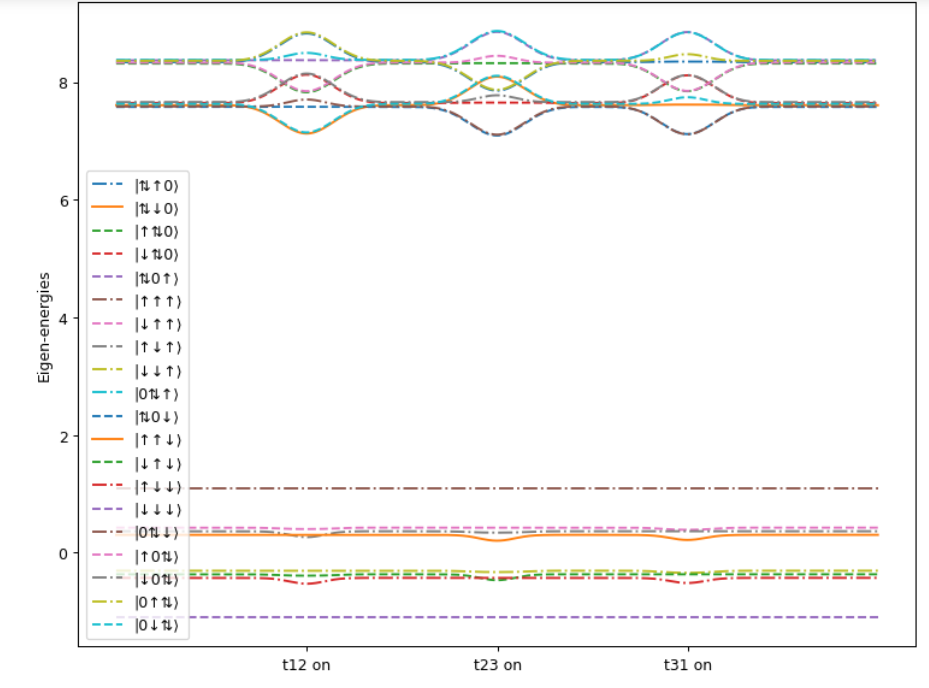
\includegraphics[scale = 0.7]{Figures/Energy_levels/elevels1.png}
    \caption{The complete set of three-dot, three-electron energy levels when the $t_{12}$,$t_{23}$ and $t_{31}$ coupling constants are increased in sequence. This diagram is intended to show the structure of the states; the energies are given in arbitrary units.}
    \label{fig:alllevels}
\end{figure}
\begin{figure}[ht]
    \centering
    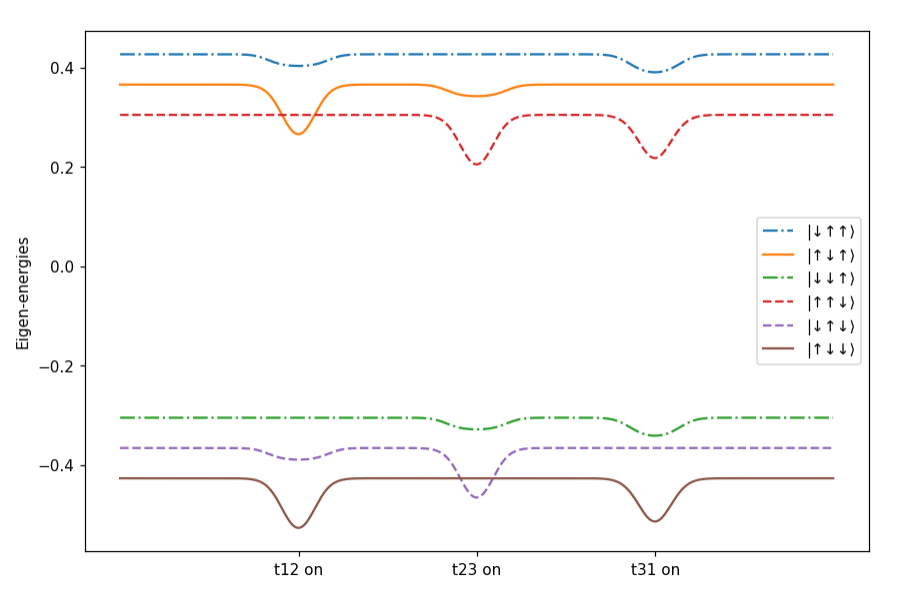
\includegraphics[scale = 0.7]{Figures/Energy_levels/elevels2.png}
    \caption{A zoomed view of figure \ref{fig:alllevels}: the computational basis states that undergo energy shifts when the coupling constants are increased in sequence. As in figure \ref{fig:alllevels}, the energies are given in arbitrary units.}
    \label{fig:complevels}
\end{figure}

Note that $\epsilon = 1$ gives the standard \texttt{CZ} gate. To implement this gate, we apply a voltage `pulse' to the inter-qubit gates in order to adjust the $t_{ij}$. Figure \ref{fig:alllevels} shows all $\binom{6}{3} = 20$ energy levels (eigenvalues of the Hamiltonian) for a three-dot, three-electron system. The higher energy set of states are those states with two electrons on one site (incurring a coulomb energy penalty of $U_i$) and can be disregarded using a Schrieffer-Wolf transformation \cite{bravyi_2011}, such that we use only the remaining 8 eigenstates as our computational basis states. The adjustments to just those computational basis states that undergo energy shift are shown in figure \ref{fig:complevels}. We see that `turning on' $t_{ij}$ results in energy levels $i$ and $j$ shifting down in energy\footnote{These levels are being repelled by the doubly occupied states with which they are coupled, but they also repel each other, hence the lower state deflects more than the upper one in each pair, the latter effect being least apparent in the $i = 1, j = 3$ case where the energy levels are furthest apart.}. By turning on this perturbation adiabatically, we cause the computational levels to shift into these lower levels and hence accrue a phase shift relative to the phase they would have accrued had they not been perturbed. It should be noted that the shift experienced by, for example, the $\ket{\downarrow\uparrow\uparrow}$ state during a $t_{12}$ pulse is identical to the deflection of the $\ket{\downarrow\uparrow\downarrow}$ and so both of these states will accrue a phase shift (in the interaction picture) of 
\begin{equation*}
    \ket{\downarrow\uparrow\uparrow} \rightarrow e^{-i\phi_1} \ket{\downarrow\uparrow\uparrow}
\end{equation*}
\begin{equation*}
    \ket{\downarrow\uparrow\downarrow} \rightarrow e^{-i\phi_1} \ket{\downarrow\uparrow\downarrow}
\end{equation*}
\begin{equation*}
    \phi_1 = \frac{1}{\hbar}\int_{T_0}^{T_1}{(E(t) - E_0)dt}
\end{equation*} where $E(t)$ and $E_0$ are the perturbed and stationary energies of the $\ket{\downarrow\uparrow\uparrow}$ state (or equivalently of the $\ket{\downarrow\uparrow\downarrow}$ state). The $\ket{\uparrow\downarrow\uparrow}$ and $\ket{\downarrow\uparrow\uparrow}$ are analagously shifted by a phase $\phi_2$. From now on we will use quantum information notation and identify $\ket{...\uparrow...} \rightarrow \ket{...0...}$, and $\ket{...\downarrow...} \rightarrow \ket{...1...}$. We represent the state of a system as a vector:
\begin{equation*}
\ket{\Psi} = 
    \begin{bmatrix}
    \alpha_{000} \\\alpha_{001} \\\alpha_{010} \\\alpha_{011} \\\alpha_{100} \\\alpha_{101} \\\alpha_{110} \\\alpha_{111} \\
    \end{bmatrix} \cdot
    \begin{bmatrix}
    \ket{000} \\\ket{001} \\\ket{010} \\\ket{011} \\\ket{100} \\\ket{101} \\\ket{110} \\\ket{111} \\
    \end{bmatrix} \cdot
\end{equation*}
in which notation the perturbation takes the unitary form
\begin{equation*}
    U_\mathrm{Pert} = 
    \begin{bmatrix}
        1 & 0 & 0 & 0 & 0 & 0 & 0 & 0\\
        0 & 1 & 0 & 0 & 0 & 0 & 0 & 0\\
        0 & 0 & e^{-i\phi_1} & 0 & 0 & 0 & 0 & 0\\
        0 & 0 & 0 & e^{-i\phi_1} & 0 & 0 & 0 & 0\\
        0 & 0 & 0 & 0 & e^{-i\phi_2} & 0 & 0 & 0\\
        0 & 0 & 0 & 0 & 0 & e^{-i\phi_2} & 0 & 0\\
        0 & 0 & 0 & 0 & 0 & 0 & 1 & 0\\
        0 & 0 & 0 & 0 & 0 & 0 & 0 & 1\\
    \end{bmatrix}
\end{equation*}
To turn this into a \texttt{CPHASE}, we apply two additional $R^z$ single-qubit rotations using microwave drives, specifically
\begin{equation*}
    R^z_1(\phi_1) = R^z(\phi_1) \otimes I \otimes I
\end{equation*}
\begin{equation*}
    R^z_2(\phi_2) = I \otimes R^z(\phi_2) \otimes I
\end{equation*}
which then give a total unitary of 
\begin{equation*}
     U^{\texttt{CPHASE}}_{12}(\epsilon) = 
     \begin{bmatrix}
        1 & 0 & 0 & 0 & 0 & 0 & 0 & 0\\
        0 & 1 & 0 & 0 & 0 & 0 & 0 & 0\\
        0 & 0 & 1 & 0 & 0 & 0 & 0 & 0\\
        0 & 0 & 0 & 1 & 0 & 0 & 0 & 0\\
        0 & 0 & 0 & 0 & 1 & 0 & 0 & 0\\
        0 & 0 & 0 & 0 & 0 & 1 & 0 & 0\\
        0 & 0 & 0 & 0 & 0 & 0 & e^{i(\phi_1 + \phi_2)} & 0\\
        0 & 0 & 0 & 0 & 0 & 0 & 0 & e^{i(\phi_1 + \phi_2)}\\
    \end{bmatrix}
\end{equation*} where we identify $\epsilon = -(\phi_1 + \phi_2)$. Since $phi_1$ and $\phi_2$ both grow monotonically with $T$, we can in principle achieve any $\epsilon$. The same scheme works for implementing a \texttt{CPHASE} gate for any pair of qubits, although the times $T$ must be tuned separately for each pair. A CPHASE gate is implemented in the simulation software I wrote in figure \ref{fig:benchmark} in chapter \ref{chap:methods}.

\chapter{Decoherence theory}\label{appendix:decoherence}
Decoherence in qubits is commonly decomposed into two main channels: phase damping and amplitude damping. Amplitude damping is concerned with processes of relaxation that cause a qubit in the higher energy $\ket{1}$ state (in my project this is represented with a spin-up electron on a qubit) to the $\ket{0}$ state. Since these states have different energies, this process is asymmetrical: relaxation requires emission of a photon and occurs at a higher rate than the reverse process\cite{Loss2022}, electron promotion via absorption. 

Amplitude damping has Krauss operators (see, e.g. \cite{Nielsen2010}):
\begin{align*}
E_0 &= \begin{bmatrix}
1 & 0\\
0 & \sqrt{1-\gamma} 
\end{bmatrix}   &   E_1 &= \begin{bmatrix}
0 & \sqrt{\gamma}\\
0 & 0 
\end{bmatrix}\\
\end{align*}
where gamma can be thought of as the probability that a photon is lost in the time interval the Krauss operators describe. These have the following effect on a density matrix:
\begin{equation*}
    \begin{bmatrix}
        \rho_{00} & \rho_{01} \\ \rho_{10} & \rho_{11}
    \end{bmatrix}
    \longrightarrow
    \begin{bmatrix}
        \rho_{00} + \gamma \rho_{11} & \sqrt{1-\gamma} \rho_{01} \\ \sqrt{1-\gamma} \rho_{10} & (1-\gamma) \rho_{11}
    \end{bmatrix}
\end{equation*}
The other decoherence channel of interest is phase damping. This is the channel we must worry about if we wish to preserve the fidelity of electrons in a $\ket{+} = (\ket{0} + \ket{1})/\sqrt{2}$ state, as its rate is generally much greater than that of amplitude damping in silicon. Intuitively, one imagines where stray and unknown EM fields shift the relative energies of the $\ket{1}$ and $\ket{0}$ states, resulting in a phase drift of the qubits over time, which, for our ignorance of the specifics, we might model as Brownian motion:
\begin{equation*}
\alpha\ket{0} + \beta\ket{1} \longrightarrow \alpha\ket{0} + \exp(-i W(\Delta t) \sqrt{2\lambda}) \beta\ket{1}
\end{equation*}
where $W(\Delta t)$ is a Wiener process, that is, a Gaussian random variable with units of $t^{1/2}$ with $\mathbf{E}[W(\Delta t)] = 0$ and $\mathbf{Var}[W(\Delta t)] = \Delta t$. $\lambda$ is the rate of wander with units of inverse time. This process results in a transformation on a general density matrix:
\begin{equation} \label{eq:phasedamptrans}
    \begin{bmatrix}
        \rho_{00} & \rho_{01} \\ \rho_{10} & \rho_{11}
    \end{bmatrix}
    \longrightarrow
    \begin{bmatrix}
        \rho_{00} & e^{-\Delta t \lambda} \rho_{01} \\ e^{-\Delta t \lambda} \rho_{10} & \rho_{11}
    \end{bmatrix}
\end{equation} or using Krauss operators:
\begin{align*}
E_0 &= \begin{bmatrix}
1 & 0\\
0 & e^{-\Delta t \lambda}
\end{bmatrix}   &   E_1 &= \begin{bmatrix}
0 & 0\\
0 & \sqrt{1-e^{-2\Delta t \lambda}}
\end{bmatrix}\\
\end{align*}
This process, although apparently qualitatively different, is mathematically equivalent to a Poisson `phase-flip' process with rate $\lambda$, in which case we have
\begin{equation*}
\alpha\ket{0} + \beta\ket{1} \longrightarrow 
\begin{cases} 
      \alpha\ket{0} - \beta\ket{1} & p\\
      \alpha\ket{0} + \beta\ket{1} & 1-p \\
   \end{cases}
\end{equation*} where the probability of ending up flipped at the end of the time interval is
\begin{equation}\label{eq:p_def}
    p = e^{-\Delta t \lambda}\left(\frac{\lambda}{1!} + \frac{\lambda^3}{3!} \cdots\right) = \frac{1}{2}(1-e^{-\Delta t \lambda})
\end{equation}
it is then straightforward to verify this gives the same density matrix transformation as in (\ref{eq:phasedamptrans}). This equivalence gives an intuitive way of understanding the futility of attempting to preserve the state of the state undergoing Brownian phase motion through the quantum Zeno effect: measurement has no effect on states that are already an eigenstate of the measurement. Mathematically this is easiest to see by transforming to the $\ket{+}$, $\ket{-}$ basis, where a mixed state whose eigenstates are basis states transforms as follows:
\begin{align*}
    \begin{bmatrix}
        \rho_{++} & 0\\ 0 & \rho_{--}
    \end{bmatrix}
    \longrightarrow
    &\begin{bmatrix}
        \frac{1}{2}(1+e^{-\Delta t \lambda})\rho_{++} + \frac{1}{2}(1-e^{-\Delta t \lambda})\rho_{--} & 0 \\
        0 & \frac{1}{2}(1-e^{-\Delta t \lambda})\rho_{++} + \frac{1}{2}(1+e^{-\Delta t \lambda})\rho_{--}
    \end{bmatrix}\\
    = &\begin{bmatrix}
        (1-p)\rho_{++} + p\rho_{--} & 0 \\
        0 & p\rho_{++} + (1-p)\rho_{--}
    \end{bmatrix}\\
\end{align*}
In this basis we may write:
\begin{equation*}
    \rho \longrightarrow (1-p)\rho + p X\rho X
\end{equation*}
So after the decoherence has been applied, whatever the underlying process, we may consider the system to still be a purely probabilistic mixture of $\ket{+}$ and $\ket{-}$, decaying to the maximally mixed state as $\Delta t \rightarrow \infty$.

This result, which extends naturally to the $N$ qubit case, opens the door to a purely Markovian analysis of complex error correction schemes.

\subsubsection{Explanation in terms of Coherence Theory}
The theory of coherence quantification, whose development was set in motion by Baumgratz et al. in 2014\cite{Baumgratz2014}, seeks to understand quantify quantum coherence as a resource to be used up by decohering operations. The development of this theory has led to the definitions of \textit{incoherent} (from the original paper) and \textit{strictly incoherent} \cite{Yadin2016} quantum operations. The theory requires the definition of a fixed basis with respect to which coherence is measured (the $\ket{+}$ is only incoherent in the $\ket{+}$, $\ket{-}$ basis, for instance). 

An incoherent operation is defined in this theory as one that maps incoherent states, which are states that are diagonal in the chosen basis, to other diagonal states. Note that these definitions are at odds with some other definitions of incoherence and coherence in other sub-fields of quantum information research. The definition given is that for an operation defined by Krauss operators $\{E_\mu\}$, for each of the $E_\mu$:
\begin{equation*}
    E_\mu \sum_i p_i \ket{i}\bra{i} E_\mu^\dag = \sum_i q_i \ket{i}\bra{i}
\end{equation*}
While not mentioned by the authors, it is straightforward to show that the property of incoherence of an operation, in contrast to the property of incoherence of a \textit{state}, is unitarily invariant, that is, an operation that is incoherent in one basis is necessarily incoherent in all others. In addition, it is obvious that an operation whose Krauss operators are chosen from the (possibly scaled) Krauss operators of other incoherent operators is itself incoherent. Within this framework it is easy to see why amplitude damping, bit-flip (both manifestly incoherent in the computational basis), phase flip (manifestly incoherent in the $\ket{+}$, $\ket{-}$ basis), and phase-bit flip (manifestly incoherent in the $(\ket{0} \pm i\ket{1})/\sqrt{2}$ basis) channels as well as combinations of the above such as the depolarising channel are all incoherent operations. Of these, the amplitude damping and bit-flip channels are further \textit{strictly incoherent}, meaning the measurement statistics of the state after their application are independent of the off-diagonal elements of the state prior to the application. The theory of quantifying coherence then requires that any useful measure of coherence monotonically decrease under the application of these operations. In our case, we start in a incoherent state, so for all such measures $\mathcal{C}$, we have $\mathcal{C}(\rho_0) = 0$, which remains true for all subsequent time.

\chapter{Change of basis to regard the codespace as one state}\label{appendix:changeofbasis}
To simplify the analysis of the 3 qubit phase-flip Shor code treated in section \ref{sec:repeat_analysis}, we perform a state-dependent, \textit{non-unitary} transformation that allows us to treat any state in the codespace as a single basis state. This results in an \textit{underestimate} of the error-correction performance of the scheme, which is detailed in this appendix.

The state to be protected is
\begin{equation*}
    \ket{\psi} = \alpha \ket{0} + \beta \ket{1},
\end{equation*} which we have encoded as
\begin{equation*}
    \rightarrow \alpha \ket{000} + \beta \ket{111}.
\end{equation*}
We assume that $\alpha \neq \beta$ (see later). To examine the dynamics of this states, we will transform to the following `analytical' basis:
\begin{align*}
    \alpha \ket{000}+ \beta \ket{111} &\longrightarrow \ket{000}\\
    \alpha \ket{111}+ \beta \ket{000} &\longrightarrow \ket{111}\\
    \alpha \ket{001}+ \beta \ket{110} &\longrightarrow \ket{001}\\
    \alpha \ket{110}+ \beta \ket{001} &\longrightarrow \ket{110}\\
    \alpha \ket{010}+ \beta \ket{101} &\longrightarrow \ket{010}\\
    \alpha \ket{101}+ \beta \ket{010} &\longrightarrow \ket{101}\\
    \alpha \ket{100}+ \beta \ket{011} &\longrightarrow \ket{100}\\
    \alpha \ket{011}+ \beta \ket{100} &\longrightarrow \ket{011}.
\end{align*}
This is not a unitary transformation. However, all of the error operations and correction unitaries we make use of take the form of Z gates (phase flips) in the computational basis, which are invariant under the transformation given above. Measurements of parity are also invariant under this transformation. The only relevant calculation not invariant under this transformation is calculation of the fidelity. This reflects reality: the effectiveness of any such error correction scheme varies greatly with the state being protected. The state $(\ket{000} + \ket{111})/\sqrt{2}$ breaks this transformation as it maps to both $\ket{000}$ and $\ket{111}$ - that it, it is identical to itself with all its phases flipped. Hence no matter how many error flips occur, the correction scheme can push the state back to exactly the correct state with at most one correction flip.

This effect can be quantified: if the target state in the `analytical' basis is $\ket{000}$, then if those states are occupied with probabilities $\{P_i\}$, then the fidelity in this basis is simply $P_0$. However, this means the actual state of the qubits is $\alpha \ket{000} + \beta \ket{111}$ with probability $P_0$, and in $\alpha \ket{111} + \beta \ket{000}$ with probability $P_7$, with a (generally small) probability of being in another state. Given the target state to be protected in this basis is $\alpha \ket{+++} + \beta \ket{---}$, the actual fidelity is:
\begin{align*}
    F = P_0 + P_7|\alpha^* \beta + \beta^* \alpha|^2 = P_0 + \left[\lvert\braket{0|\psi}\rvert^2 - \lvert\braket{1|\psi}\rvert^2\right]^2P_7
\end{align*}
Integrating the value of this expression over the surface of the Bloch sphere, one obtains an `average' fidelity of $P_0 + 2P_7/3$. I am not sure how useful this metric is however, and in any case, in most error correction schemes of interest, we have at all times $P_0 + P_7 \approx 1$, so this is only really a linear correction. The analysis of section \ref{sec:repeat_analysis} proceeds in the `analytical' basis given above, taking $P_0$ at the relevant metric.

\chapter{Markovian analysis of repeated error correction schemes}\label{appendix:markovanalysis}
\subsubsection{Modelling readout fidelities}
Readout for quantum dot qubits always involves some form of \textit{spin to charge conversion} as the interaction of the spins themselves with the environment is weak (this is why the $T_1$ times for these systems are so good). Spin to charge conversion involves some form of tunneling process, of which the simplest form is Elzerman readout, where spin-up and spin-down electrons tunnel to a reservoir with different tunneling rates, which we define as $\gamma$ for spin up electrons, resulting from an odd parity state between the relevant qubits, and $\Gamma$ for spin down electrons. Techniques such as RF reflectometry also involve waiting for some form of electron tunnelling event, so this model could potentially be used to describe these techniques as well. For an effective scheme, we expect that $\gamma \gg \Gamma$.

From these we can calculate the chance that we detect a tunneling event given that the ancilla is spin up $F_1$ and the chance that there is no tunneling event detected given the electron is spin down $F_0$. A perfect scheme would have $F_0 = F_1 = 1$. A simple model for these readout times, assuming the amplitude relaxation time $T_1 \gg \Gamma^{-1}, \gamma^{-1}$ is (simplified from \cite{Keith2019}):
\begin{align*}
    F_0 &= e^{-\Delta t \Gamma} & F_1 &= 1-e^{-\Delta t \gamma}
\end{align*}
\subsubsection{Error matrix and correction matrix}
Thanks to the results of the first section (the density matrix remains diagonal) we may treat the correction step entirely classically. For example, if we find ourselves in the $\ket{001}$ state after the error step, we will measure an even parity on qubits 0 and 1 with probability $F_0$ and an odd parity on qubits 1 and 2 with probability $F_1$. If we perform both of these measurements correctly, we will ascertain that we are in the even-odd subspace and we need to flip qubit 2, returning us to the $\ket{000}$ state. If, however, the $A_{12}$ ancilla qubit electron fails to tunnel out in time, we will believe that we are still in the even-even subspace, and no correction step will be taken. Similarly, there eventualities (of varying probability) that will lead to any one (or none) of the three qubits being flipped by the correction processor. For this state, the full complement of options is:
\begin{equation*}
\ket{001} \longrightarrow 
\begin{cases} 
      \ket{000} F_0 F_1 \\
      \ket{001} F_0 F_1' \\
      \ket{011} F_0' F_1 \\
      \ket{101} F_0' F_1'
   \end{cases}
\end{equation*}
with $F_0' = 1-F_0$, $F_1' = 1-F_1$.

Before continuing to write the whole evolution matrix like this, there is a simplification one can make: the states $\ket{001}$ and $\ket{100}$ behave identically: for every state that could follow from either state (other than the states themselves) these two states have the same probability of transitioning to it. The same goes for the pair of states $\ket{011}$ and $\ket{110}$. We therefore choose to define a single probability for each of these pairs of states, and not care which of the two it inhabits. The error matrix can also be modified to accommodate this amalgamation, meaning that out system is now one of 6-dimensional vectors rather than 8-dimensional vectors.

With this in mind, we can describe the error step as:
\begin{equation} \label{eq:Ematrix}
    \begin{bmatrix}
        P_0(t+\Delta t) \\
        P_1(t+\Delta t) + P_4(t+\Delta t) \\
        P_2(t+\Delta t) \\
        P_5(t+\Delta t) \\
        P_6(t+\Delta t)  + P_3(t + \Delta t)\\
        P_7(t+\Delta t) \\
    \end{bmatrix}
    =
    \begin{bmatrix}
        q^3& q^2p& q^2p& qp^2& qp^2& p^3 \\
        2 q^2p& qp^2 + q^3& 2 qp^2& 2 q^2p& p^3 + q^2p& 2 qp^2\\
        q^2p& qp^2& q^3& p^3& q^2p& qp^2\\
        qp^2& q^2p& p^3& q^3& qp^2& q^2p\\
        2 qp^2& p^3 + q^2p& 2 q^2p& 2 qp^2& q^3 + qp^2& 2 q^2p\\
        p^3& qp^2& qp^2& q^2p& q^2p& q^3\\

    \end{bmatrix}
    \begin{bmatrix}
        P_0(t) \\
        P_1(t) + P_4(t) \\
        P_2(t) \\
        P_5(t) \\
        P_6(t)  + P_3(t)\\
        P_7(t) \\
    \end{bmatrix}
\end{equation}
and the correction step as
\begin{equation} \label{eq:Cmatrix}
    \begin{bmatrix}
        P_0(t+\Delta t) \\
        P_1(t+\Delta t) + P_4(t+\Delta t) \\
        P_2(t+\Delta t) \\
        P_5(t+\Delta t) \\
        P_6(t+\Delta t)  + P_3(t + \Delta t)\\
        P_7(t+\Delta t) \\
    \end{bmatrix}
    =
    \begin{bmatrix}
        F_0^2 & F_0 F_1 & F_1^2 & 0 & 0 & 0 \\
        2F_0'F_0 & F_0 F_1' & 0 & 2F_1 F_1' & F_0' F_1 & 0\\
        F_0'^2 & 0 & F_1'^2 & 0 & F_0' F_1' & 0 \\
        0 & F_0' F_1' & 0 & F_1'^2 & 0 &F_0'^2 \\
        0 &F_0' F_1 & 2F_1' F_1&0&F_0F_1'&2F_0'F_0 \\
        0&0&0& F_1^2 &F_0 F_1 & F_0^2
    \end{bmatrix}
    \begin{bmatrix}
        P_0(t) \\
        P_1(t) + P_4(t) \\
        P_2(t) \\
        P_5(t) \\
        P_6(t)  + P_3(t)\\
        P_7(t) \\
    \end{bmatrix}
\end{equation}
The evolution of the state in time in one step is given by $M = CE$ where $E$ and $C$ are the matrices defined in (\ref{eq:Ematrix}) and (\ref{eq:Cmatrix}) respectively. We prepare the system in a pure $\ket{000}$ state, $P_i = \delta_{i,0}$, and repeatedly apply $M$ to evolve the $P_i$.  




\chapter{Treatment of continuous error correction scheme using second-order perturbation theory}\label{appendix:perturbationtheory}

In this section the behaviour of the system described in \ref{chapter:CQEC} is predicted using second-order perturbation theory, along with various approximations to make the problem tractable. 

Suppose the system is initally in an arbitrary codespace state, with each of the ancilla pairs starting in triplet states:
\begin{equation*}
    \ket{\psi(t = 0)} = (\alpha\ket{\uparrow_{Q1}\downarrow_{Q2}\uparrow_{Q3}} + \beta\ket{\downarrow_{Q1}\uparrow_{Q2}\downarrow_{Q3}})(\ket{\uparrow_{A1}\downarrow_{A3}} + \ket{\downarrow_{A1}\uparrow_{A3}})(\ket{\uparrow_{A2}\downarrow_{A4}} + \ket{\downarrow_{A2}\uparrow_{A4}}) / 2
\end{equation*}
First consider the case where no coupling is applied between the qubits. If we can engineer our system so that $\delta_{1,3}^z = E_{A1}^z - E_{A3}^z \ll 1/T_1$, and similarly $\delta_{2,4}^z \ll 1/T_1$ (with $T_1$ the timescale of bit flip errors), then the energy difference between the two branches of each qubit singlet is sufficiently small that rate at which the triplets rotate into triplets, and so register a tunnelling event on the reflectometry apparatus, is long compared to the error time and so not limiting. We can see this by considering a single ancilla branch:
\begin{equation}
    \ket{\psi(t)} = \frac{1}{\sqrt{2}}(\ket{\uparrow\downarrow} + \exp(-2i\delta t)\ket{\downarrow\uparrow}) = \frac{1}{2}\ket{T_0}(1 + \exp(-2i\delta t)) + \frac{1}{2}\ket{S_0}(1 - \exp(-2i\delta t)))
\end{equation} \label{eq:triplet_to_singlet}, so that the amplitude of the singlet state goes as 
\begin{equation*}
    \left|\braket{S_0|\psi(t)}\right|^2 = \sin(\delta t)^2
\end{equation*}.

Now we apply a coupling between the following four pairs of qubits: Q1 and A1, Q2 and A1, Q2 and A2, Q3 and A2. We consider the four branches of the state in the computational basis of the ancilla qubits separately, and apply second order perturbation theory to approximate the energy shift of each state due to the adiabatic application of a weak coupling, of strength $t$. The limits of this approximate treatment will be tested using a numerical simulation developed in chapter \ref{chap:methods}.

The standard formula for second order perturbation theory is (there is no first-order shift in energy as the perturbing terms are off-diagonal):

\begin{equation*}
    E_i^1 \approx E_i^0 + \sum_j{\frac{|\braket{\psi_i|V|\psi_j}|^2}{E_i^0 - E_j^0}}
\end{equation*} where $E_i^0$ and $E_i^1$ are the unperturbed and perturbed energies of state $i$, and $H_0$ and $V$ are the basic and perturbative Hamiltonians. If we set $V$ to the hopping term in the Hubbard model, then we obtain, for example,
\begin{align*}
    E_{\uparrow\downarrow\uparrow,\uparrow\downarrow,\uparrow\downarrow}^1 - E_{\uparrow\downarrow\uparrow,\uparrow\downarrow,\uparrow\downarrow}^0 &= 
    -\frac{t^2}{E_{\uparrow\updownarrow \uparrow,\varnothing\downarrow,\uparrow\downarrow}^0 - E_{\uparrow\downarrow\uparrow,\uparrow\downarrow,\uparrow\downarrow}^0}
    -\frac{t^2}{E_{\uparrow\varnothing \uparrow,\updownarrow\downarrow,\uparrow\downarrow}^0 - E_{\uparrow\downarrow\uparrow,\uparrow\downarrow,\uparrow\downarrow}^0}
    -\frac{t^2}{E_{\uparrow\updownarrow \uparrow,\uparrow\downarrow,\varnothing\downarrow}^0 - E_{\uparrow\downarrow\uparrow,\uparrow\downarrow,\uparrow\downarrow}^0}
    -\frac{t^2}{E_{\uparrow\varnothing \uparrow,\uparrow\downarrow,\updownarrow\downarrow}^0 - E_{\uparrow\downarrow\uparrow,\uparrow\downarrow,\uparrow\downarrow}^0}\\
    &= -t^2\left(\frac{1}{\Delta_1} + \frac{1}{\Delta_2} + \frac{1}{\Delta_3}+ \frac{1}{\Delta_4}\right)
\end{align*} with
\begin{align*}
    \Delta_1 &= U_{Q2} + \mu_{Q2} - \mu_{A1} + \E_{Q2}^z - \E_{A1}^z \\
    \Delta_2 &= U_{A1} + \mu_{A1} - \mu_{Q2} + \E_{Q2}^z - \E_{A1}^z \\
    \Delta_3 &= U_{Q2} + \mu_{Q2} - \mu_{A2} + \E_{Q2}^z - \E_{A2}^z \\
    \Delta_4 &= U_{A2} + \mu_{A2} - \mu_{Q2} + \E_{Q2}^z - \E_{A2}^z \\
\end{align*}, where the terms describe parameters of the Hubbard model described in section \ref{sec:hubbard_model}.

We note that $U_i \gg \Delta \mu_i, E^z_i$, and that the magnitude of $U_i$ (order of a few \unit{\milli\electronvolt}) varies little from site to site , so that we may define $\Lambda_t = 2t^2/\braket{U_i}$. Then we have 
\begin{equation*}
    E_{\mathrm{C}\uparrow\downarrow,\uparrow\downarrow}^1 - E_{\mathrm{C}\uparrow\downarrow,\uparrow\downarrow}^0  = \Delta E_{\mathrm{C}\uparrow\downarrow,\uparrow\downarrow} \approx
    \Delta E_{\mathrm{C}\uparrow\downarrow,\downarrow\uparrow} \approx
    \Delta E_{\mathrm{C}\downarrow\uparrow,\uparrow\downarrow} \approx
    \Delta E_{\mathrm{C}\downarrow\uparrow,\downarrow\uparrow} \approx -2\Lambda_t
\end{equation*}, where we note the shift in energy is the same, within the above approximations, for both of the codespace branches, $\ket{\uparrow\downarrow\uparrow}$ and $\ket{\downarrow\uparrow\downarrow}$, and denote the energies of both branches by the subscript C. All branches of the ancilla state will therefore accrue phase at the same rate as long as the state code qubits remains within the codespace.

\newcommand{\dlam}[2]{\diagbox{$#1\Lambda_t$}{$#2\Lambda_t$}}
\begin{table}
    \centering
\begin{tabular}{|c|c||c|c|c|c|}
\hline
\multicolumn{2}{|c||}{Computational branch} & \multicolumn{4}{c|}{Ancilla branch} \\
\hline
 Subspace & branch & $\uparrow\downarrow\uparrow\downarrow$ & $\uparrow\downarrow\downarrow\uparrow$ & $\downarrow\uparrow\uparrow\downarrow$ & $\downarrow\uparrow\downarrow\uparrow$ \\
 \hhline{|=|=||=|=|=|=|}

Codespace & \diagbox{$\uparrow\downarrow\uparrow$}{$\downarrow\uparrow\downarrow$} & $2\Lambda_t$ & $2\Lambda_t$ & $2\Lambda_t$ & $2\Lambda_t$\\
\hline
E1 & \diagbox{$\downarrow\downarrow\uparrow$}{$\uparrow\uparrow\downarrow$} & \dlam{3}{1} & \dlam{3}{1} & \dlam{1}{3} & \dlam{1}{3}\\
\hline
E2 &\diagbox{$\uparrow\uparrow\uparrow$}{$\downarrow\downarrow\downarrow$} & \diagbox{$0$}{$4\Lambda_t$} & $2\Lambda_t$ & $2\Lambda_t$ & \diagbox{$4\Lambda_t$}{$0$}\\
\hline
E3 & \diagbox{$\uparrow\downarrow\downarrow$}{$\downarrow\uparrow\uparrow$} & \dlam{3}{1} & \dlam{1}{3} & \dlam{3}{1} & \dlam{1}{3}\\
\hline
\end{tabular}
\caption{Table of the (negative) energy shifts due to coupling of each ancilla branch, of each computational branch, of each subspace.}\label{table:shifts}
\end{table}


When a bit-flip error occurs, the state will acquire a component in one of the error subspaces, denoted E1, E2 and E3 depending on which qubit has flipped. Applying the above analysis, we calculate the energy shifts of each of the ancilla branches of each computational branch in each codespace. These are given in table \ref{table:shifts}. These shifts result in the A1, A3, or A2, A4 ancilla pairs rotating from triplets to singlets, or both, depending on the error subspace. To see this, consider the E1 error subspace, into which the state moves when the Q1 qubit experiences a bit-flip error. If both ancilla pairs are in triplet states at the point when the system transitions into the E1 subspace from the codespace, the state undergoes the following evolution \footnote{We assume that the resultant state is approximately a stationary state of the perturbed Hamiltonian.}:

\begin{align*}
    \ket{\psi(t)} = &\alpha\ket{\downarrow\downarrow\uparrow}(
        e^{-3 i \Lambda_t t }\ket{\uparrow\downarrow\uparrow\downarrow} 
    + e^{-3 i \Lambda_t t }\ket{\uparrow\downarrow\downarrow\uparrow}
    + e^{-i \Lambda_t t }\ket{\downarrow\uparrow\uparrow\downarrow}
    + e^{-i \Lambda_t t }\ket{\downarrow\uparrow\downarrow\uparrow})/2 \\
    + e^{-i\delta_{Q1,Q3} t} &\beta\ket{\uparrow\uparrow\downarrow}(
        e^{- i \Lambda_t t }\ket{\uparrow\downarrow\uparrow\downarrow} 
    + e^{- i \Lambda_t t }\ket{\uparrow\downarrow\downarrow\uparrow}
    + e^{-3i \Lambda_t t }\ket{\downarrow\uparrow\uparrow\downarrow}
    + e^{-3i \Lambda_t t }\ket{\downarrow\uparrow\downarrow\uparrow})/2 \\
    &\approx e^{-3 i \Lambda_t t}\alpha\ket{\downarrow\downarrow\uparrow}
    (\ket{\uparrow\downarrow} + e^{2 i \Lambda_t t }\ket{\downarrow\uparrow})
    (\ket{\uparrow\downarrow} + \ket{\downarrow\uparrow})/2 \\
    &+ e^{- i \Lambda_t t}\beta\ket{\uparrow\uparrow\downarrow}
    (\ket{\uparrow\downarrow} + e^{-2 i \Lambda_t t }\ket{\downarrow\uparrow})
    (\ket{\uparrow\downarrow} + \ket{\downarrow\uparrow})/2
\end{align*}, where the $\delta_{Q1, Q3}$ phase term accounts for the difference in energy between the two branches, which is small compared to $\Lambda_t$, and irrelevant to our conclusion, so we ignore it. By comparison with equation \ref{eq:triplet_to_singlet}, we see that the A1,A3 ancilla pair in both branches will rotate into a triplet state with a characteristic timescale $1/\Lambda_t$. The same analysis yields for E2 error subspace:
\begin{align*}
    \ket{\psi(t)} \approx &\alpha\ket{\downarrow\downarrow\uparrow}
    (\ket{\uparrow\downarrow} + e^{ -2 i \Lambda_t t }\ket{\downarrow\uparrow})
    (\ket{\uparrow\downarrow} + e^{ -2 i \Lambda_t t }\ket{\downarrow\uparrow})/2 \\
    + e^{-4 i \Lambda_t t} &\beta\ket{\downarrow\downarrow\uparrow}
    (\ket{\uparrow\downarrow} + e^{ 2 i \Lambda_t t }\ket{\downarrow\uparrow})
    (\ket{\uparrow\downarrow} + e^{ 2 i \Lambda_t t }\ket{\downarrow\uparrow})/2
\end{align*}, so that both pairs of ancillas rotate into singlets. The E3 case is identical to the E1 case with the appropriate qubits exchanged, and leads to only the A2, A4 qubit pair rotating into a singlet.

\subsection{Further questions related to tunnelling physics} \label{sec:tunneling_question}

Much work has been done optimising the implementation and examining the classical physics of reflectometry as a tool for quantum measurement. For a review see \cite{Vigneau2023}, especially section VIII. During the project the author has not had time to study the physics behind this technique in detail. It appears, however, that present analyses treat the system semi-classically in assuming that an electron tunnels, or does not, within the measurement period (i.e. the period of time that the tunneling barrier between the pair of qubits is lowered). They then seek to maximise the fidelity with which this charge-shifting event, or lack thereof, is detected. This tunneling event is interpreted as a projective measurement of the singlet/triplet system at the point of measurement, with probabilities of either state given by Born's rule. In the present case this is an insufficient analysis: at any given time, there is necessarily some finite component of the electron pair state that is a singlet, and we need to establish a rate at which tunnelling occurs as a function of the amplitude of this component. A full treatment of this problem probably needs to be formulated in terms of quantum master equations and the theory of quantum decoherence \cite{Wiseman1996}.

Time has not permitted me to look into this issue, so at the suggestion of my supervisor I will make the simplifying assumption that any ancilla pair that acquires more than a 10\% square-amplitude of singlet immediately tunnels and is hence registered by the dispersive readout device with empirically determined fidelity.

\chapter{Using alternative codespaces for continuous error correction}\label{appendix:evenparitycodespace}

\begin{figure}[ht]
    \centering
    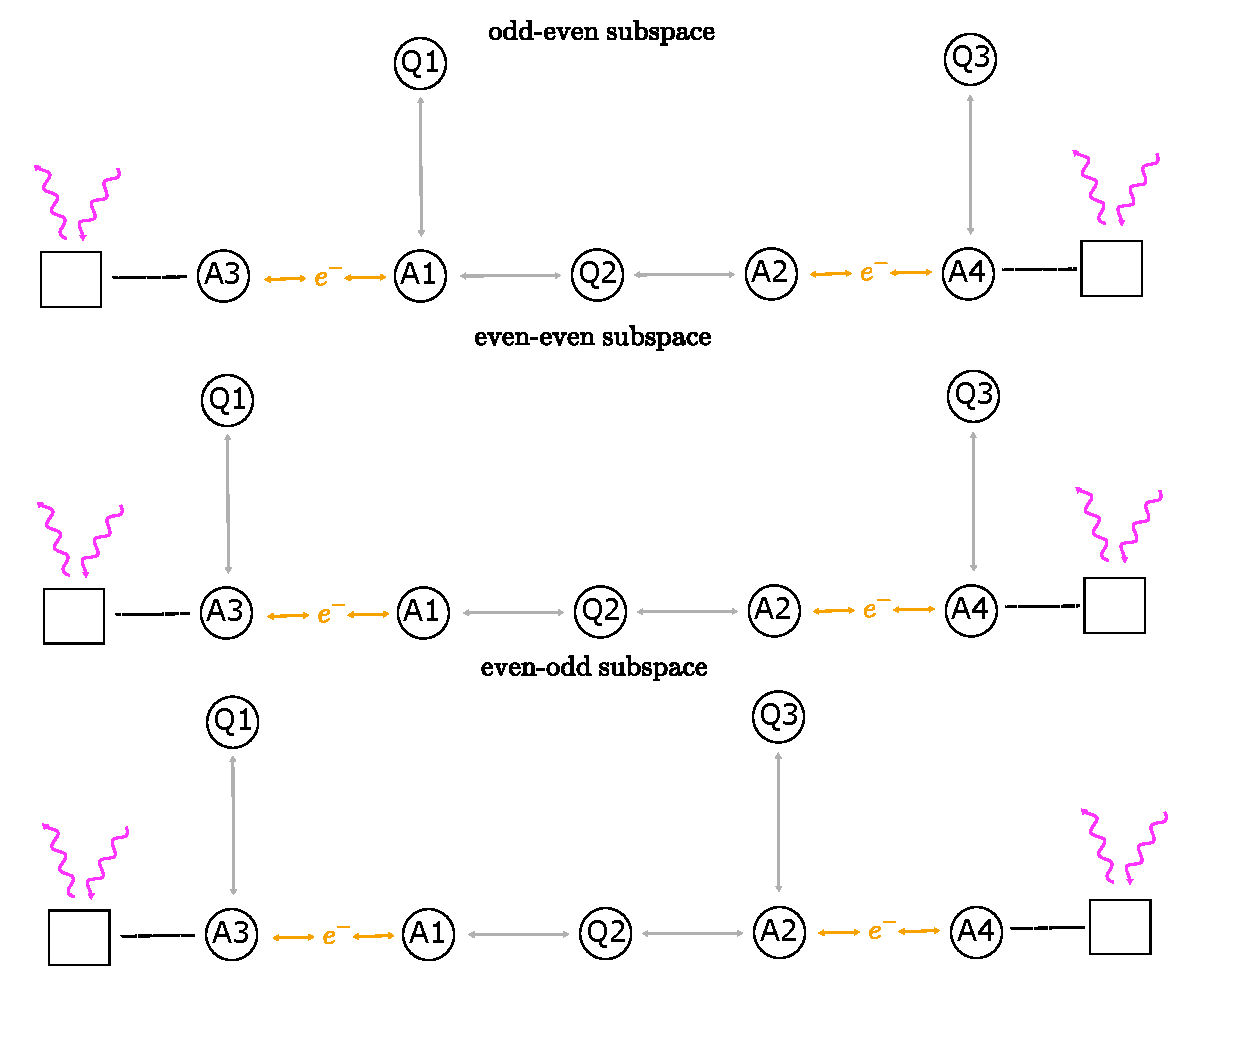
\includegraphics[scale = 0.9]{Figures/different_codespaces.pdf}
    \caption{The modified qubit layouts that would allow for the use of the odd-even, even-even and even-odd parity subspaces as the codespaces.}
    \label{fig:differentcodespaces}
\end{figure}
It is possible to use an alternative subspace of the space of code qubit states as the codespace for the error-correction scheme rather than the odd-odd parity subspace as described in section \ref{sec:truly_continuous_theory}. This requires a modification to the circuit layout. For example, to use the even-even subspace as the codespace, qubits Q1 and Q2 must be coupled to A1 and A3 respectively, and Q2 and Q3 to A2 and A4 respectively. This is shown in the central panel of figure \ref{fig:differentcodespaces}, which can be compared with figure \ref{fig:7qubitlayout}. Then the second-order perturbation theory analysis follows that of section \ref{sec:truly_continuous_theory}, but with a modified table of energy shifts, given here as table \ref{table:evenshifts}. This leads to behaviour entirely analogous to the behaviour with the odd-odd parity used as the subspace.

Further work is needed to examine if there is an advantage to using one subspace over another. For the purposes of this project, it was most practical to examine the odd-odd codespace as it leaves qubits A3 and A4 uncoupled to the other qubits, which allows an approximate basis reduction, making simulations much easier (section \ref{sec:reduced_basis_approx}). This freedom to configure the qubits in various ways may be useful in experimental work with constraints on the positioning of circuit elements/the topology of the circuit.

This freedom leads to an interesting possibility. The standard approach in QEC is to apply correction flips when a parity measurement collapses the state into an error-space. An alternative approach is to \textit{not} apply a correction flip, but rather \textit{redefine the codespace} to the newly inhabited subspace and modify the circuit that is being executed dynamically and interpret the circuit output based on the knowledge of what subspace the qubits inhabit. One could achive this with a modified version of the present scheme, where a controller changes whether Q1 is coupled to A1 or A3, and whether Q3 is coupled to A2 or A4, when an error occurs. This would stabilise the qubits in the new sub-space. The system does not have to apply a correction flip, whose application might lead to additional errors.

\begin{table}
    \centering
\begin{tabular}{|c|c||c|c|c|c|}
\hline
\multicolumn{2}{|c||}{Computational branch} & \multicolumn{4}{c|}{Ancilla branch} \\
\hline
 Subspace & branch & $\uparrow\downarrow\uparrow\downarrow$ & $\uparrow\downarrow\downarrow\uparrow$ & $\downarrow\uparrow\uparrow\downarrow$ & $\downarrow\uparrow\downarrow\uparrow$ \\
 \hhline{|=|=||=|=|=|=|}

Codespace & \diagbox{$\uparrow\uparrow\uparrow$}{$\downarrow\downarrow\downarrow$} & $2\Lambda_t$ & $2\Lambda_t$ & $2\Lambda_t$ & $2\Lambda_t$\\
\hline
E1 & \diagbox{$\downarrow\uparrow\uparrow$}{$\uparrow\downarrow\downarrow$} & \dlam{3}{1} & \dlam{3}{1} & \dlam{1}{3} & \dlam{1}{3}\\
\hline
E2 & \diagbox{$\uparrow\downarrow\uparrow$}{$\downarrow\uparrow\downarrow$}& $2\Lambda_t$ &\diagbox{$0$}{$4\Lambda_t$}& \diagbox{$4\Lambda_t$}{$0$} & $2\Lambda_t$ \\
\hline
E3 & \diagbox{$\uparrow\uparrow\downarrow$}{$\downarrow\downarrow\uparrow$} & \dlam{1}{3} & \dlam{3}{1} & \dlam{1}{3} & \dlam{3}{1}\\
\hline
\end{tabular}
\caption{Modified version of table \ref{table:shifts} showing the shifts when the circuit is set up to use the even-even subspace as the codespace.}\label{table:evenshifts}
\end{table}



\chapter{Detecting errors in ancilla qubits} \label{appendix:9qubitsystem}
One problem the error correction scheme described in section \ref{sec:truly_continuous_theory} is that it is entirely vulnerable to errors occurring in the ancilla qubits. If one such error did occur, the system would assume the resulting tunneling event was a result of a code qubit error and apply an erroneous correction gate, which would then push the system irreversibly out of the codespace.
\begin{figure}[ht]
    \centering
    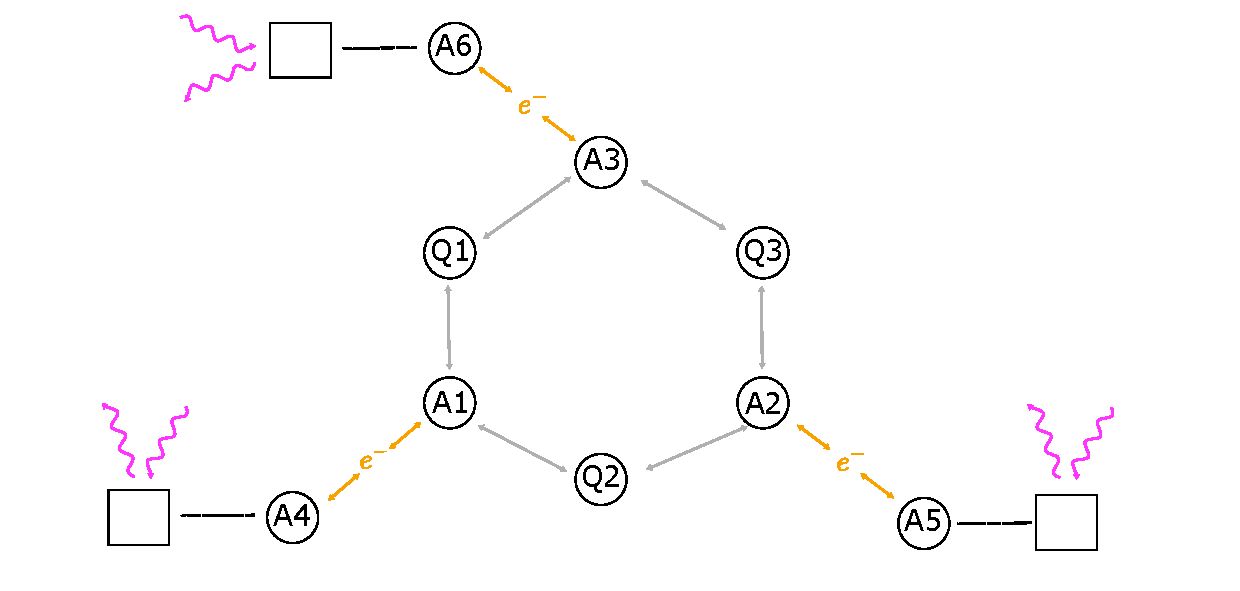
\includegraphics[scale = 0.9]{Figures/9q.pdf}
    \caption{The modified qubit layout that would allow for detection of ancilla errors.}
    \label{fig:9qubitlayout}
\end{figure}
Figure \ref{fig:9qubitlayout} shows a layout that incorporates redundancy into the ancilla measurements. With this setup, the system would always expect to see two ancilla tunneling events in case of an error in the code qubits. If only one tunneling event was detected, the system could assume that the error was only in the that ancilla system, and reset it without taking the code qubits out of the codespace.

The limitation in implementing a scheme such as this one is at present topological; there has not yet been any experimental demonstration of 2D qubits arrays large enough for such a system.
\chapter{Locked states} \label{appendix:lockedstates}
The purpose of this section a system that is continuously sensitive to both phase- and bit-flip errors. I will describe a set of what I call `locked states' which have the property that either a spin or phase flip results in an immediately visible charge movement, and suggest a highly theoretical outline of an error correction scheme for qubit storage. I suspect this scheme is highly impractical, but it is mathematically interesting.

\subsubsection{Bit-flip only scheme}
The idea presented in this subsection is due to Chris Long, a PhD candidate at the Cavendish and Hitachi Laboratory.
Consider a line of three qubits, with charge sensors coupled to each end. We encode the qubit state $\alpha \ket{0} + \beta\ket{1}$ as $\alpha \ket{000} + \beta\ket{111}$. If we apply a strong enough permanent potential difference so that the middle quantum dot has a lower chemical potential than the outer ones, then the system would be able to lower its energy by significantly shifting the system wavefunction to have a substantial component with double occupation on the middle qubit, that is, the states $\ket{\dots \updownarrow \dots}$. Colloquially, the electrons will 'want' to tunnel onto the middle qubit. However, the Pauli exclusion principle prevents them from doing so, as in each branch of the wavefunction all three electrons have the same spin. When one of the qubits changes state from up to down, however, one or both of the outer qubits (depending on which electron flipped) will be free to tunnel. This should be visible through the charge detector. It is not clear how possible it is to then reset the qubit to the codespace whilst preserving the encoded qubit. In any event, this scheme does not protect against phase-flip errors.
\subsubsection{Locked states}
The following are my own invention (as far as I know). Consider the $n$-qubit states ($n \ge 3$) defined by
\begin{align*}
    \ket{L0} &= \sqrt{\frac{2}{2^N}}\left[\sum_{n_1(s) = 0\mathrm{\ mod}4}{\ket{s}} - \sum_{n_1(s) = 2\mathrm{\ mod}4}{\ket{s}}\right] \\
    \ket{L1} &= \sqrt{\frac{2}{2^N}}\left[\sum_{n_1(s) = 0\mathrm{\ mod}1}{\ket{s}} - \sum_{n_1(s) = 2\mathrm{\ mod}3}{\ket{s}}\right]
\end{align*} where $n_1(s)$ is the number of $1$s that appear in the bit-string representation of state $\ket{s}$.

For example, for $n = 3$ we have
\begin{align*}
    \ket{L0} &= (\ket{000} - \ket{011} - \ket{101} - \ket{110})/2 \equiv (\ket{\uparrow\uparrow\uparrow} - \ket{\uparrow\downarrow\downarrow} - \ket{\downarrow\uparrow\downarrow} - \ket{\downarrow\downarrow\uparrow})/2\\
    \ket{L1} &= (-\ket{111} + \ket{100} + \ket{010} + \ket{001})/2 \equiv (-\ket{\downarrow\downarrow\downarrow} + \ket{\downarrow\uparrow\uparrow} + \ket{\uparrow\downarrow\uparrow} + \ket{\uparrow\uparrow\downarrow})/2
\end{align*}. The $n=3$ case is most relevant for physical systems, but the mathematical properties given here are general. Note
\begin{itemize}
    \item These two states are orthogonal $\braket{L0|L1} = 0$, so linear combinations of them can encode a qubit.
    \item All electron hopping in this system is forbidden by either Pauli or triplet blockade. The state has no coupling to any doubly occupied state in the Fock basis, regardless of which hopping terms in a Hubbard Hamiltonian are switched on.
\end{itemize}

\begin{figure}[ht]
    \centering
    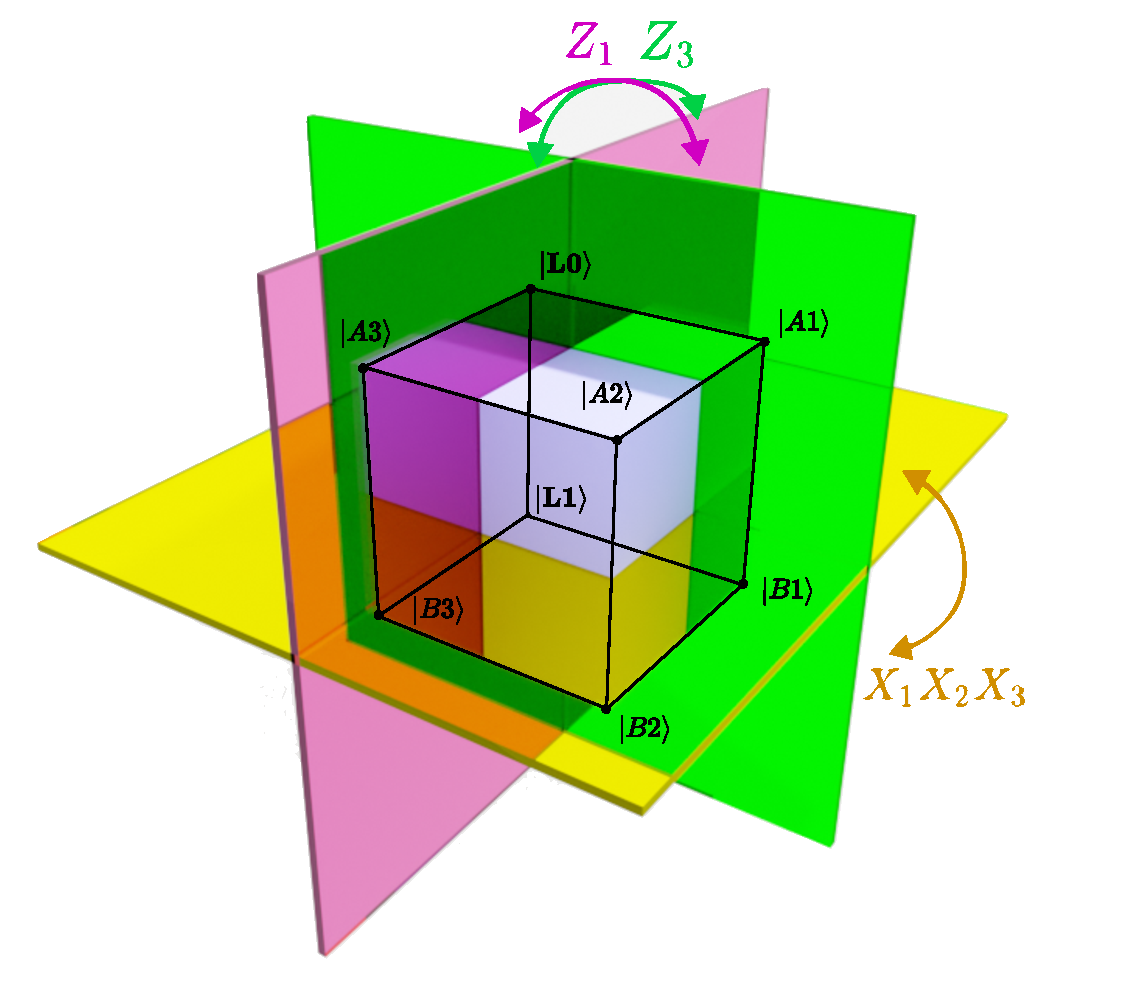
\includegraphics[scale = 0.6]{Figures/group/group.pdf}
    \caption{Group structure of the $n=3$ locked states and error states. Starting from the locked states, phase and bit-flip errors with a combination of reflections in the planes shown.
    }\label{fig:group}
\end{figure}
Now suppose a bit-flip or error flip occurs on any of the qubits. Then 
\begin{align*}
    Z_1\ket{L0} = -X_1\ket{L1} = &(\ket{000} - \ket{011} + \ket{101} + \ket{110})/2 = \ket{A1}\\
    X_1\ket{L0} = Z_1\ket{L1} = &(\ket{100} - \ket{111} + \ket{001} + \ket{010})/2 = \ket{B1}
\end{align*} with $\ket{A2},\ket{A3},\ket{B2},\ket{B3}$ defined similarly. The three generators of the group $\mathbb{Z}_2\times\mathbb{Z}_2\times\mathbb{Z}_2$ can be mapped to $Z_1, Z_3$ and $X_1X_2X_3$ which defines a representation of this group acting on the 3 qubit Hilbert space. The 8 group elements can be mapped to the identity, the three phase-flips, the three bit-flips, and a triple-bit-flip that takes $\ket{L0}$ to $\ket{L1}$, an instantaneous process for which there would be no clear mechanism. It is clear, therefore, that any combination of these errors will keep the state within this set of states.

\begin{figure}[ht]
    \centering
    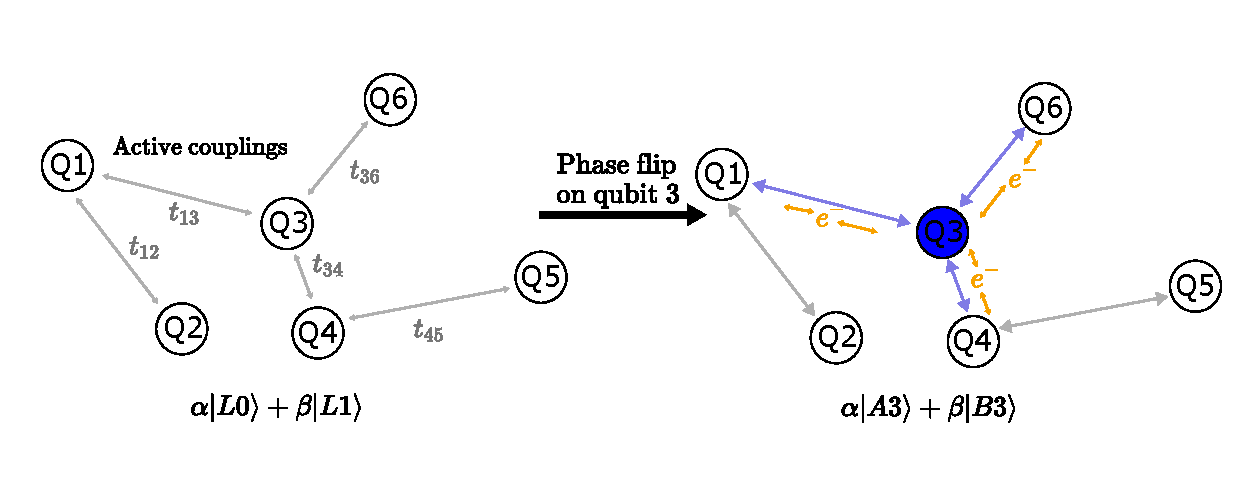
\includegraphics[scale = 0.8]{Figures/locked_states.pdf}
    \caption{The locked property of a locked state. In the codespace, spanned by $\ket{L0}$ and $\ket{L1}$, no electrons can `move' (i.e. the state is uncoupled to the doubly occupied states). If, for example, a phase flip occurs on qubit 3, then the state moves into the $\ket{A3}, \ket{B3}$ error subspace. In this subspace, electrons are free to hop between qubit 3 and the neighbouring qubits where there is a coupling applied. This can perhaps be detected by a charge sensor.
    }\label{fig:lockedstates}
\end{figure}

The states $\ket{Ai}$ and $\ket{Bi}$ have the property that turning on the hopping term in the Hubbard Hamiltonian between qubit $i$ and any other qubit $j$ will now result in a non-zero coupling to the relevant doubly occupied states. If a potential difference is applied to encourage tunneling, this double occupation will be registered on a charge sensor. The nature of the wavefuntion collapse in this case is somewhat unclear.
\subsubsection{Creating the locked states}
Despite their apparent complexity, these states can be created using a quantum circuit with depth that is linear in the number of qubits. I will give the $n$-qubit circuit, and illustrate the effects for clarity on the $n = 3$ case.

Start with a single ancilla qubit and the n qubits which we want to turn into a locked state and apply a Hadamard gate to each of this latter group:
\begin{equation*}
    \ket{0}\ket{000}\xrightarrow{H^{\otimes n}} \ket{0}(\ket{000} + \ket{001} + \ket{010} + \ket{011} + \ket{100} + \ket{101} + \ket{110} + \ket{111})/\sqrt{8}
\end{equation*}.
Then apply a $Rz(\pi/2)$ rotation to every qubit:
\begin{equation*}
    \xrightarrow{Rz(\pi/2)^{\otimes n}} \ket{0}(\ket{000} + i\ket{001} + i \ket{010} - \ket{011} + i \ket{100} - \ket{101} - \ket{110} -i \ket{111})/\sqrt{8}
\end{equation*}. Now apply controlled X gates, conditioned on each qubit and targeting the ancilla:
\begin{align*}
    \xrightarrow{\prod_i^\otimes{CX(i,0)}} &\frac{\ket{0}}{4}(\ket{000} - \ket{011} - \ket{101} - \ket{110})
    + \frac{i\ket{1}}{4}(\ket{001} + \ket{010} + \ket{100} - \ket{111})\\
    = &\frac{\ket{0}}{\sqrt(2)}\ket{L0} + \frac{i\ket{1}}{\sqrt(2)}\ket{L1}
\end{align*}. We now need to configure this into a general linear combination of $\ket{L0}$ and $\ket{L1}$.
\begin{align*}
    \xrightarrow{Rz_0(-\pi/2)} &\frac{\ket{0}}{\sqrt(2)}\ket{L0} + \frac{\ket{1}}{\sqrt(2)}\ket{L1}\\
    \xrightarrow{\prod_i^\otimes{CX(0,i)}} & \frac{\ket{0} + \ket{1}}{\sqrt{2}}\ket{L0}\\
    \xrightarrow{U} & (\alpha\ket{0} + \beta\ket{1})\ket{L0}\\
    \xrightarrow{\prod_i^\otimes{CX(i,0)}} & \alpha\ket{0}\ket{L0} + \beta\ket{1}\ket{L1}
\end{align*}
\subsubsection{Error detection and correction}
It is clear from the above how these locked states could be used for an error detection scheme. It is less clear to what extent these states could be used for error correction. An outline scheme could be:
Start with two groups of qubits, each in a locked state, with no $t$ coupling between them, in the codespace:
\begin{equation*}
    \ket{\psi(0)} = \alpha\ket{L0}\ket{L0} + \beta\ket{L1}\ket{L1}
\end{equation*}. Now suppose a phase flip occurs in the second qubit of the second group of qubits:
\begin{align*}
    \xrightarrow{Z_2,2} &\alpha\ket{L0}\ket{A2} + \beta\ket{L1}\ket{B2}\\
    =&\alpha\ket{L0}(-\ket{1\mathbf{01}} + \ket{111} + \ket{1\mathbf{10}}+\ket{011})/2 + \beta\ket{L1}(-\ket{0\mathbf{10}} + \ket{000} + \ket{0\mathbf{01}}+\ket{100})/2.
\end{align*}
This allows electrons to hop between qubits 1 and 2, and between 2 and 3 of the second group. The component of double occupation should cause the system to collapse into a charge eigenstate with double occupation on one of the three qubits. If the system then relaxes back into the computational basis, perhaps due to the potential difference being lowered, the only trace of which type of error occurred will remain on the unaffected qubit in the second group. In the example above, the charge hops between qubits 2 and 3 of the second group (in bold). The single occupation states must collapse away, and we are left with, after relaxation:
\begin{align*}
    \rightarrow\alpha\ket{L0}\ket{110} + \beta\ket{L1}\ket{010}.
\end{align*}. We can use an ancilla qubit and a series of $CX$ gates with the qubits of the first locked state to find out which error occurred:
\begin{align*}
    \xrightarrow{\text{ancilla}} & \ket{0}(\alpha\ket{L0}\ket{110} + \beta\ket{L1}\ket{010})
    \xrightarrow{\prod_i^\otimes CX(i,0)}\alpha\ket{0}\ket{L0}\ket{110} + \beta\ket{1}\ket{L1}\ket{010}
\end{align*}. We can then apply the following projective measurement:
\begin{align*}
    P_1 = \ket{00}\bra{00} + \ket{11}\bra{11} && P_2 = \ket{01}\bra{01} + \ket{10}\bra{10}
\end{align*}
where the first and second qubit represent the ancilla qubit and the first qubit of the second group respectively. This tells us the error syndrome, and it is just a matter of applying more $CX$ gates following the construction procedure detailed above to return the system to the codespace.

\chapter{Hubbard model Hamiltonian simulator}\label{appendix:software}

In this appendix I discuss some of the more interesting details of the software I wrote to simulate the Hubbard model. A substantial portion of the time of the project went into the design and implementation of this simulator.

\subsubsection{Python extension: \texttt{FastHamiltoniser}}
This section will discuss the methodology used to perform simulations of scheme described in section \ref{sec:truly_continuous_theory} on a Hubbard model of a multiple quantum dot system. The treatment of the error correction scheme described in section \ref{sec:truly_continuous_theory} is necessarily highly approximate due to the complexity of the high-dimensional Hilbert space involved (for 7 electrons on 7 sites, the occupation basis is of dimension 3432) and the large number of parameters of the Hubbard model, so makes multiple simplifying assumptions, chiefly the application of second-order perturbation theory and ignoring the site-to-site variance in certain model parameters. It is therefore valuable to simulate the Hubbard model numerically to test the validity of these assumptions in various parameter regimes.

My supervisor Dr. Arvidsson-Shukur and his collegues have developed a code (yet unpublished), \texttt{DotHamiltoniser}, designed to generate Hubbard Hamiltonians in an occupation basis given a set of physical parameters ($E_i^z, U_i$, etc.), as well as to perform low-dimensional time-evolution simulations. This was very helpful at the start of my project to visualise the energy levels of the system and their dependence on coupling. However, it was not designed for higher dimensional time evolution, and could not be used for this purpose due to performance limitations.

I therefore designed a Hamiltonian simulation code, inspired by the work of Dr Arvidsson-Shukur et al., with the ability to handle higher dimensional systems. The system has three main components: 
\begin{enumerate}
    \item A python extension, \texttt{FastHamiltoniser}, written in C, C++ and CUDA, which provides highly performant specialised sparse matrix operations for use in Hamiltonian time evolution. This stores and updates the Hamiltonian as a set of sparse \texttt{Permuter} objects to improve performance.
    \item \texttt{Hamiltonian}, a python class that builds a Hubbard model Hamiltonian from physical parameters. This implements all the relevant second-quantised physical calculations necessary for Hubbard model, building the $n$ site, $m$ electron Fock basis as a set of bit strings and defining raising and lowering operators, projector matrices, unitary matrices, etc. in this basis.
    \item \texttt{Evolution}, a python class which takes as input a Hamiltonian and a set of continuous time instructions, which are defined as recursive composite instructions, to produce a time evolution of a given starting statevector.
\end{enumerate}

\begin{figure}[ht]
    \centering
    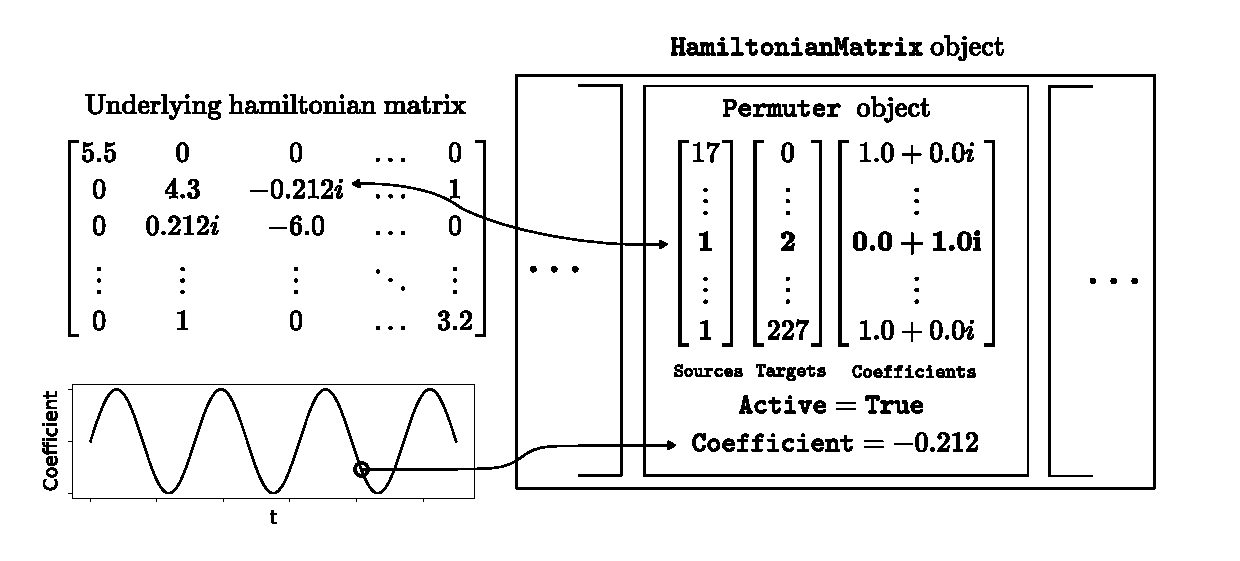
\includegraphics[scale = 0.8]{Figures/fasthamiltoniser/diagram.pdf}
    \caption{How sparse Hamiltonian matrices are represented in the custom python extension \texttt{FastHamiltoniser}. The non-zero matrix elements are grouped into objects of type \texttt{Permuter}, whose structure is calculated in advance but whose activation and multiplicative coefficients are modified efficiently as runtime.}
    \label{fig:fasthamiltoniser}
\end{figure}
\subsubsection{Structure of extension}
The purpose of the simulator is to solve the Schrödinger equation
\begin{equation} \label{eq:schrodinger}
    \dot{\psi} = -i H \psi 
\end{equation} (here expressed in natural units $\hbar = 1$) where $\psi$ is a vector in the occupation basis of a Hubbard Hamiltonian. In order to use Runge-Kutta \cite{Butcher1996} methods of integration, we need to be able to calculate this derivative efficiently at an arbitrary time and with arbitrary input. $H$ is typically very sparse, with the only off-diagonal terms given by magnetic drives and hopping couplings, of which typically only a subset of size linear in the number of qubits are non-zero at a given time. 

To perform this calculation efficiently, I implemented the following data structure in C. A \texttt{HamiltonianMatrix} object, illustrated in figure \ref{fig:fasthamiltoniser}, contains basic data about the dimension of the array, as well as an array of pointers to objects of type \texttt{Permuter}. Each of these \texttt{Permuter} objects stores three arrays of equal length, two of integers representing source and target vector indices, and one of floats representing matrix coefficients, where each entry represents a matrix element. \texttt{Permuter}s also store a complex coefficient, which can be changed over time by writing to a single variable, and a boolean representing whether it is `on' or `off'. The internal arrays are determined in advance of the simulation by python code, and thereafter only the strength and activations of the \texttt{Permuter} objects need be modified during the simulation. For example, one such object provides all the on-diagonal elements of the matrix, and another might provide all the off-diagonal elements associated with a particular J-coupling between two qubits.

The calculation \ref{eq:schrodinger} can then be performed by iterating over the active permuters and building up the derivative vector according to the permutation and coefficient arrays. 
\subsubsection{Interaction picture calculation}
A further requirement that favoured the development of a custom C backend was the ability to perform simulations in the interaction picture. Performing simulations in the interaction picture is necessary due to the large differences in energy between eigenstates, for example due to the $U_i$ on-site repulsion in some states. With any choice of reference energy in a static basis, there are always states whose phase rotate much faster than the timescale of the evolutions that I wish to simulate, meaning there is no suitable step-size that captures the desired phenomena within reasonable computational time with the simulation remaining stable. Instead, we perform the following transformation to the interaction picture:
\begin{align*}
    \dot{\psi_i} &= -i\sum_j{H_{ij}\psi_j}\\
     \psi_i \rightarrow \phi_i &= e^{-i H_{ii} t} \psi_i \\
    \Rightarrow \dot{\phi} &= -i\sum_{j\ne i}{e^{- i (H_{jj} - H_{ii})t} H_{ij}\phi_j}
\end{align*}.

Since most off-diagonal terms $H_{ij}$ are zero at most points in time, this results in most states being stationary and lowering the rate of rotation of affected states to a longer timescale that can be simulated. It introduces the additional complexity, however, of introducing a time-dependence into the Hamiltonian. I wrote a C function to perform the modified matrix multiplication, calculating the phase factors as required.

\subsubsection{GPU acceleration}
The calculation to be performed is parallel in nature, and thus a candidate for GPU acceleration. I wrote the requisite kernels\footnote{This presented a lot of technical challenges as the process for incorporating CUDA C++ into python C extensions and compiling them is not documented and very technical. I made a template project with the setup to use in the future: https://github.com/Stasiu51/TemplateCudaEx} to perform the matrix multiplication in CUDA, a variant of C++ developed by Nvidia to control their graphics processing units (`GPU's) \cite{cuda}, one of which (a P620 Quadro) is installed in my laptop. On testing, the CUDA variant outperformed the CPU calculation only for systems with more than around 15 qubits, more than required and where the speed of computation is too slow for practical use anyway ($<10$ iterations per second, several orders of magnitude too slow for the simulations of the present project).

\subsubsection{Python class for Hubbard model construction: \texttt{Hamiltonian}}
This is a python class (and supporting code) that implements a Hubbard Hamiltonian, using \texttt{FastHamiltoniser} as a backend to store the underlying matrix. In particular it
\begin{enumerate}
    \item creates a list of basis vectors, represented as bit strings (with convenience functions for printing them in canonical notation), that span the Fock basis of a system with a specified number of sites and number of electrons;
    \item defines creation and annihilation operators on these states, which it uses to
    \item construct the diagonal \texttt{Permuter} object that represents the self-energy terms due to chemical potential, coulomb repulsion, and static magnetic z-fields; and to
    \item construct the off diagonal \texttt{Permuter} objects generated by hopping terms and x and y magnetic fields. It also
    \item provides transformations to and from the interaction picture; and
    \item provides functions for creating projector and X matrices in the Fock basis, which are more involved to calculate than in the computational (single electron per site) basis. 
\end{enumerate}

\subsubsection{Python class for time evolution of statevector: \texttt{Evolution}}

This class takes a reference to a \texttt{Hamiltonian} object, and a set\footnote{There is in fact only one such object, as they are defined in a recursive tree structure.} of objects that subclass the abstract base class \texttt{TimeStep} whose role is to provide instructions as to how to modify the parameters of the Hubbard model at given time. For example, one such object instructs the simulation to ramp a set of hopping couplings to a specified value over a given period of time, and another might oscillate the strength of the x component of the applied magnetic field at a given frequency and phase.

The \texttt{scipy} routine \texttt{solve\_ivp} is used along with the calculations of the derivative described above in a Runge-Kutta 5th order \cite{Butcher1996} integration routine to calculate the evolution of a given initial statevector. The routine is designed to estimate the errors and dynamically choose a step size for the integration. This works poorly in the present use case, as the calculated (vector-norm) error scales with the number of non-zero elements of the vector. Instead, the code allows the user to manually specify a step size, typically around $1/10$ of the smallest relevant timescale of the system, and checks the continued normalisation of the statevector as an imperfect check on the stability of the simulation.

\subsection{Simulating the 7 qubit continuous error correction scheme} \label{sec:reduced_basis_approx}
The software enables us to set up a qubit basis that explicitly models the qubit layout shown in \ref{fig:7qubitlayout}, with three code qubits and two pairs of ancilla qubits. This 7 qubit system has a Fock basis of dimension 3432, which is just about feasible to simulate using the software I developed (simulations of sufficiently small time-step take several minutes each, and there are memory limitations in storing the results). However, this can be sped up by noting that in the circuit to be simulated, the second of each pair of ancillas, A3 and A4, do not experience any coupling, so the Hamiltonian is always diagonal in these dimensions. Furthermore, the ancilla part of all states that are non-zero in the simulation are constructed out of the $\ket{\uparrow\downarrow}$ and $\ket{\downarrow\uparrow}$ states with respect to these pairs of qubits, as well as non-computational states. Therefore, we may reduce our basis if we make an appropriate modification to the Hamiltonian:
\begin{align*}
    \ket{\dots \uparrow\downarrow\uparrow\downarrow} &\rightarrow \ket{\dots \uparrow\uparrow} &
    \ket{\dots \uparrow\downarrow\downarrow\uparrow} &\rightarrow \ket{\dots \uparrow\downarrow}\\
    \ket{\dots \downarrow\uparrow\uparrow\downarrow} &\rightarrow \ket{\dots \downarrow\uparrow} &
    \ket{\dots \downarrow\uparrow\downarrow\uparrow} &\rightarrow \ket{\dots \downarrow\downarrow}\\
    E_{A1}^z &\rightarrow E_{A1}^z - E_{A3}^z & E_{A2}^z &\rightarrow E_{A2}^z - E_{A4}^z
\end{align*} this does not affect the energy levels of the computational states, and only affects the non-computational basis states by a quantity of order $E_i^z \ll U_i$. If we accept this approximation, we can reduce our basis size to 252, which increases the simulation speed by a factor of around $14 - 20\times$ (this is a non-linear speedup as all the simulation data now fits into memory).

Also note that most variation in spin energy from site to site come from variation in the electron G factor at different sites rather than inhomogeneities in the magnetic field \cite{Hwang2017}. It is convenient and equivalent, however, to simply include these variations into the magnetic field\footnote{Although my software does have the capability to vary the electron g-factor from site to site, it is simpler not to use it. }

\end{appendices}

\printbibliography
\end{document}